\documentclass{jarticle}
\usepackage{rsjletter}
\usepackage[dvipdfmx]{graphicx}
\usepackage[dvipdfmx]{color}
\usepackage{url}
\usepackage{bm}
\usepackage{here}
%\usepackage{tikz}


\begin{document}
\title{物体の高さ方向の学習による単純形状物体の姿勢推定精度向上}
\author{○上田 純矢（名城大学）\ \ 田崎 豪（名城大学）}
%\abstract{From 2023, authors are encouraged to write an article's abstract in either Japanese or English. Ab-stracts should be 3-6 lines long (100 words or less in English). If authors use simultaneous submission of the [Letter], an abstract in English is required. If authors are not using simultaneous submission and will submit the article in English to other journals in the future, an abstract in English is not recommended due to the risk of being considered self-plagiarism. }
\abstract{PYNet has imporoved the accuracy of pose estimation for simple-shaped objects by initially estimating the object's grounding surface. 
        This approach reduces the degrees of freedom in the pose to be estimated.
         However, estimating poses that are 180°rotated remains a challenging task. 
         To address this problem, we developed a new method that also estimates the height direction of the object.
         This additional constraint on the pose of the simple-shaped object being estimated further improves the pose estimation accuracy. 
         When compared to the conventional PYNet, our method achieved an accuracy improvement of 2.41pt in the original RGBD camera dataset
        and 2.78pt in the pubic YCB object dataset. }
\setlength{\baselineskip}{4.4mm}	% 行間の設定
\maketitle
\thispagestyle{empty}
\pagestyle{empty}

\section{はじめに}
自動運転における事故防止を目的とした障害物回避のた
めに障害物を認識し，自車から障害物までの距離を推定す
る必要がある．自動運転車でよく用いられる距離センサは
LiDAR(Light Detection and Ranging)である．しかし，
LiDAR は高価であり，メンテナンスに手間がかかる．そこ
で本研究では安価な単眼カメラによる障害物検出を目的と
する．

単眼カメラによる深度推定法として NDDepth\cite{1}や
MIMDepth\cite{2}などがある．しかし，これらの手法は単眼
カメラ画像のみで深度を推定するため，推定結果を実距離
にするスケールパラメータが不定であり，正確な距離を推
定することは困難である．以降，スケールが特定された深
度を距離，スケールが特定されていない深度を単に深度と
して区別して使用する．

単眼カメラ画像に加えて，自動運転用に作成された三次
元地図\reffig{3Dmap}を入力に用いることで，障害物までの距
離を推定できるPMOD-Net\cite{3}がある．正確な距離情報を
持つ三次元地図により，PMOD-Net は単眼カメラ画像で正
確な距離を推定しつつ障害物検出が可能である．

PMOD-Net は，三次元地図と単眼カメラ画像を入力とし
て，Semantic Segmentation と距離推定をマルチタスク
に行う．Semantic Segmentation で三次元地図上に存在
しない人や車などの動的障害物を検出することにより，距
離推定タスクで動的障害物の距離も推定可能にした．しか
し，三次元地図は動的障害物の距離情報を持たないため，
地図上に存在する障害物の距離推定精度に比べて，動的障
害物の距離推定精度は低い．そこで本研究は，単眼カメラ
を用いて，三次元地図上に存在しない動的障害物までの距
離を推定するという課題に取り組む．
\begin{figure}[t]
  \centering
  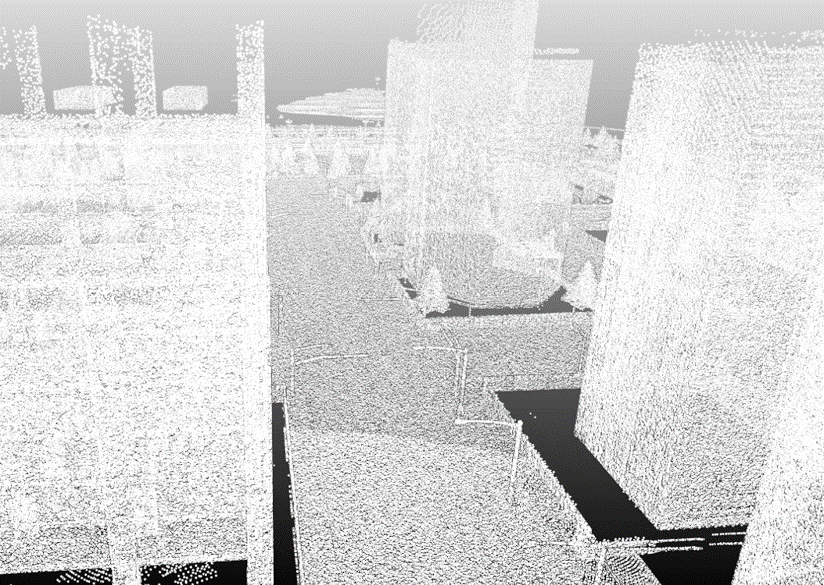
\includegraphics[width=0.95\linewidth]{img/intro/3Dmap.png}
  \caption{3D map}
  \label{3Dmap} 
\end{figure}

課題を解決するために，地図を使用する距離推定と地図
を使用しない深度推定の相補的な関係に着目した．三次元
地図を利用するPMOD-Net は距離を推定できるが，地図
の影響で動的障害物に対する距離推定精度は低い．地図を
使用しないNDDepth やMIMDepth は深度しか推定できないが，
動的障害物も含め，現在画像内にある全物体の相
対的な深度を精度よく推定できる．そこで，地図を使用し
ない単眼深度
推定法の出力を PMOD-Net へ入力する新手法 PMOD-
NetD（PMOD-Net with Depth）を開発する．三次元地
図という過去の距離情報と，単眼深度推定からの現在の深
度情報を統合し，単眼カメラによる高精度な障害物検出を
実現する．

本研究の学術的貢献は以下である．
\begin{enumerate}[1.]
  \begin{figure*}[t]
      \centering
      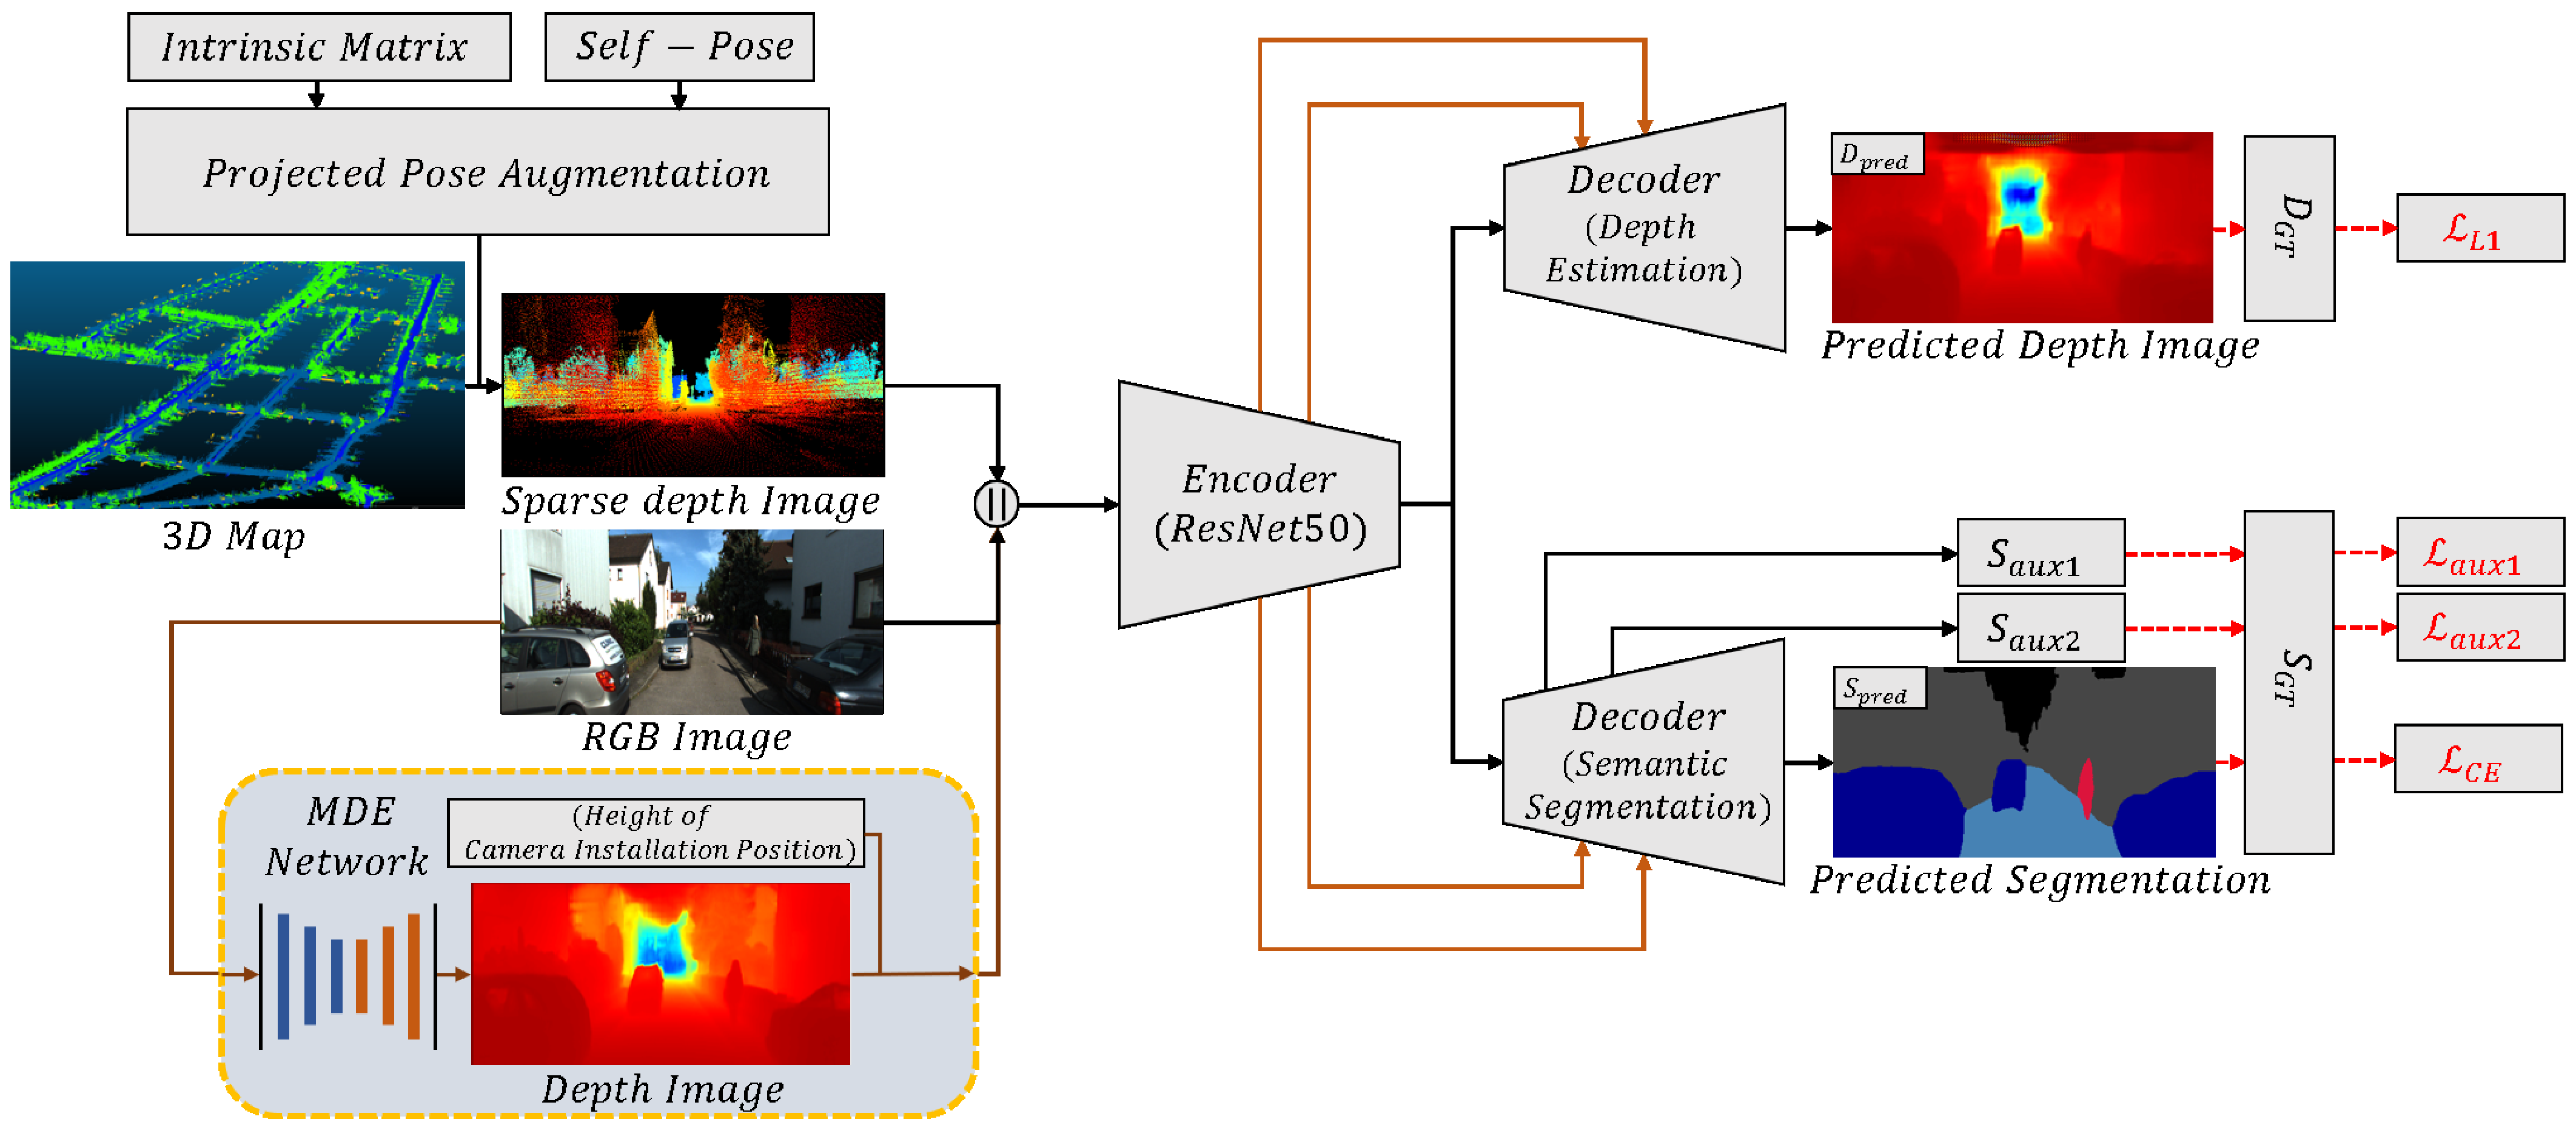
\includegraphics[width=0.95\linewidth]{img/method/network_architecture.eps}
      \caption{Network architecture of PMOD-NetD}
      \label{networkarchitecture} 
  \end{figure*}
  \item 三次元地図と単眼カメラを用いて三次元的に障害物検出を行う世界初のニューラルネットワークであるPMOD-Net を高精度化する新手法を開発した．
  \item スケールが不定であるため手法単体で扱うことが困難な単眼深度推定結果に対して三次元地図によるスケール調整が有効であることを示した．
  \item KITTI ベンチマークにおいて高順位の複数の単眼深度推定法に対して性能を高められることを確認し，手法を問わずに高精度化できる汎用性を示した．
\end{enumerate}
\section{関連研究}

\subsection{単眼深度推定}
単眼深度推定は3Dモデリング\cite{4}，ロボット工学\cite{5}，自
動運転\cite{6}などに応用され，盛んに研究されている．これら
の手法はスケールが類似した大量のデータセットで学習・
テストを行うことで，学習時と同一の環境であれば距離推
定可能である．NDDepth\cite{1}やMIMDepth\cite{2}はKITTI\cite{7}
，NYUDepth-v2\cite{8}の2 種類のデータセットにおいて高い
精度を示した．しかし，学習した環境と異なる環境では，
深度から距離へと変換するためのスケールの推定が必要と
なる．したがってスケールの推定精度によっては精度が大
きく低下する可能性がある．
\subsection{距離補完}
入力にLiDAR 点群とカメラ画像を用いてLiDAR 点群を
補完し，密な距離画像を生成する距離補完手法も多く研究
されている\cite{9}\cite{10}．三次元地図点群を疑似的なLiDAR 点
群とみなすことで，距離画像の生成が可能である．しかし，
カメラ画像とLiDAR 点群は同時刻に取得されることが前提
の手法であり，画像内の物体とLiDAR 点群は一致している
ことが望まれる．そのため三次元地図上に存在しない車や
人などの動的障害物の距離推定においてPMOD-Net\cite{3}と
同等の精度を得るのは困難である．
\subsection{PMOD-Net}
PMOD-Net\cite{3}は地図から作成した疎な距離画像とカメ
ラ画像を入力として，Semantic Segmentation と距離推
定を行う世界初のニューラルネットワークである．
Semantic Segmentation と距離推定をマルチタスクに行
うことで三次元地図上に存在しない動的障害物を含めた三
次元障害物検出を可能にした．疎な距離画像は，自己位置
推定結果をもとに三次元地図点群を画像平面に投影するこ
とで取得する．自己位置はGPS やIMU，オドメトリ，カ
メラなどで取得した値を利用する．
\subsection{本研究の位置づけ}
PMOD-Netは，単眼カメラで障害物までの正確な距離を
計測できる利点がある．さらに実際に移動ロボットで障害
物回避にも成功しているため，本研究でもベース手法とし
て使用する．本研究は，単眼カメラのみでの代表的な距離
推定手法である単眼深度推定法とPMOD-Net\cite{3}を利用す
る．しかし，双方の相補的な関係に着目し，欠点を単一
ネットワーク内で同時に解決する新手法を開発したという
点で従来とは大きく異なる．

また本研究は，開発スピードが速い単眼深度推定分野に
おいて，深度推定法そのものを開発するものではない．地
図を利用することで，深度推定法によらずに距離推定を高
精度化する手法を開発している点も，従来とは大きく異な
る．さらに従来の学習を必要としないスケー
ル調整に加えて，学習ベースでスケールを調整するという新規性があり，より高精度な距離
推定を可能にしている．




\section{提案手法}

新たに開発したPMOD-NetDの構造を\reffig{networkarchitecture}に示す．
カメラ画像から深度画像を作成し，スケール調整を行う．
ここで深度画像の作成には単眼深度推定用のニューラル
ネットワーク (Monocular Depth Estimation:MDE Network) を用いる．本研究の評価実験ではMDE
Networkとして，NDDepth\cite{1}やMIMDepth\cite{2}を用い
た．またMDE Networkが学習した環境であれば，スケー
ル調整は不要であるため，行わない．学習していない環境
であれば，スケールの調整を行う．

スケールの調整方法として，地面の高さを用いる手法
\cite{11}を利用する．地面を利用したスケール調整方法の手順
を以下に示す．
\begin{enumerate}[1.]
    \item RANSAC\cite{12}で平面推定を行い，単眼深度推定の出
    力から地面点群を抽出する．
    \item 事前に取得したカメラの高さ$z$を用いて式(\ref{Scale_S})でスケール
    $S$を算出する．ここで$P_c^{i}$と$N$はそれぞれ，単眼深度推定か
    ら得られた地面点群における点$i$の高さと点群数を示す．
    \begin{equation}
        \label{Scale_S}
        S= \frac{z}{\frac{1}{N}{}\sum_{i=1}^{N}P_c^{i}} 
    \end{equation}
\end{enumerate}

ここで取得した$S$と深度画像$I_o$からスケール調整した距離画
像$I_D$を式(\ref{metric_Id})のように取得する．
\begin{equation}
    \label{metric_Id}
    I_D=S*I_o
\end{equation}

カメラ画像と疎な距離画像，距離画像$I_D$をチャンネル方向に
結合し，PMOD-NetDの入力とする．常に絶対的な距離情報をも
つ三次元地図と入力段階で結合することで前述した欠点を補い
つつ学習を進めることができる．

また距離画像$I_D$は，任意のMDE Networkから作成可能であり，
精度が良い手法であるほど，最終的な精度を高めることができ
る．そのため，PMOD-NetとMDE Networkどちらの開発が進んで
も，精度向上に寄与することができる．
\section{評価実験}
\subsection{実験設定}
提案手法の有効性を確認するために，以下 2 つのデータ
セットで評価実験を行った．
\begin{enumerate}[1.]
  \item シミュレーションデータセット (CARLA\cite{13})
  \item 公開データ (KITTI-360 データセット\cite{14})
\end{enumerate}

どちらのデータセットにおいても，PMOD-NetDと，以下3つの手法と比較する．
\begin{enumerate}[1.]
  \item PMOD-Net\cite{3}
  \item NDDepth\cite{1}
  \item MIMDepth\cite{2}
\end{enumerate}

NDDepthとMIMDepthはKITTIデータセットで高い精度を
出しており，事前学習済みのモデルも公開されているため，
比較手法として用いることにした．学習済みのモデルが公
開されているため，KITTI-360データセットではスケール調
整不要で距離精度の比較が可能である．CARLAで使用する場
合は式(\ref{metric_Id})のようにスケール調整した結果で比較する．ここ
では2.0[m]の位置にカメラを設置した．
\subsection{使用データセット}
シミュレーションデータセットは，自動運転研究用シミュレ
ータである CARLA\cite{13}を用いて作成した．CARLAには特徴の異
なる7種類のマップがあり，マップごとにランダムに配置され
た人や車を含むデータセットを作成した．学習データには各マ
ップから600枚ずつ，合計4200枚を使用し，テストには各マッ
プから学習に使用していない1840 枚ずつ，合計12880 枚を用
いた．\reffig{ex_CARLA}に学習および評価に使用した画像例を示す．三次
元地図の投影にはシミュレータが出力するカメラ位置を用いた．
公開データセットとしてKITTI-360\cite{14}を使用した．ドイツ
郊外を撮影した大規模な車載センサデータセットであり，9つ
のシーケンスを提供している．本実験ではデータ数が少ないシ
ーケンス03を除いた8シーケンスの三次元地図と左カメラ画
像を使用した．学習データには各シーケンスから500枚ずつ，
合計4000枚を使用し，テストには学習に使用していないデー
タをすべて用いた．テスト時にはKITTI-360が提供している自
己位置誤差を含んだ慣性航法システムのデータを使用し，実際
の位置誤差を想定した実験を行った．

\subsection{評価指標}
評価は画像中の動的障害物に対して行う．本実験では人と車
を動的障害物とした．距離推定の評価指標には，距離誤差平均
を示すMAEを用いる．MAEは式(\ref{MAE})で計算する．$n$は評価対象の
領域を示す画素数であり,$i$は画素位置である．$D_P$は各手法が推
定した距離画像，$D_{GT}$は正解の距離画像である．ともにカメラか
ら各物体までの距離を示す．また方向性のあ
る誤差を評価するため，式(\ref{MAE})において絶対値内の値が正の場合と負の場合だけを評価した
値をそれぞれ ME+，ME-として分けて評価する．
\begin{equation}
  \label{MAE}
  MAE= \frac{1}{n}{}\sum_{i=1}^{n}|D_P(i)-D_{GT}(i)|
\end{equation}
\begin{figure}[t]
  \centering
  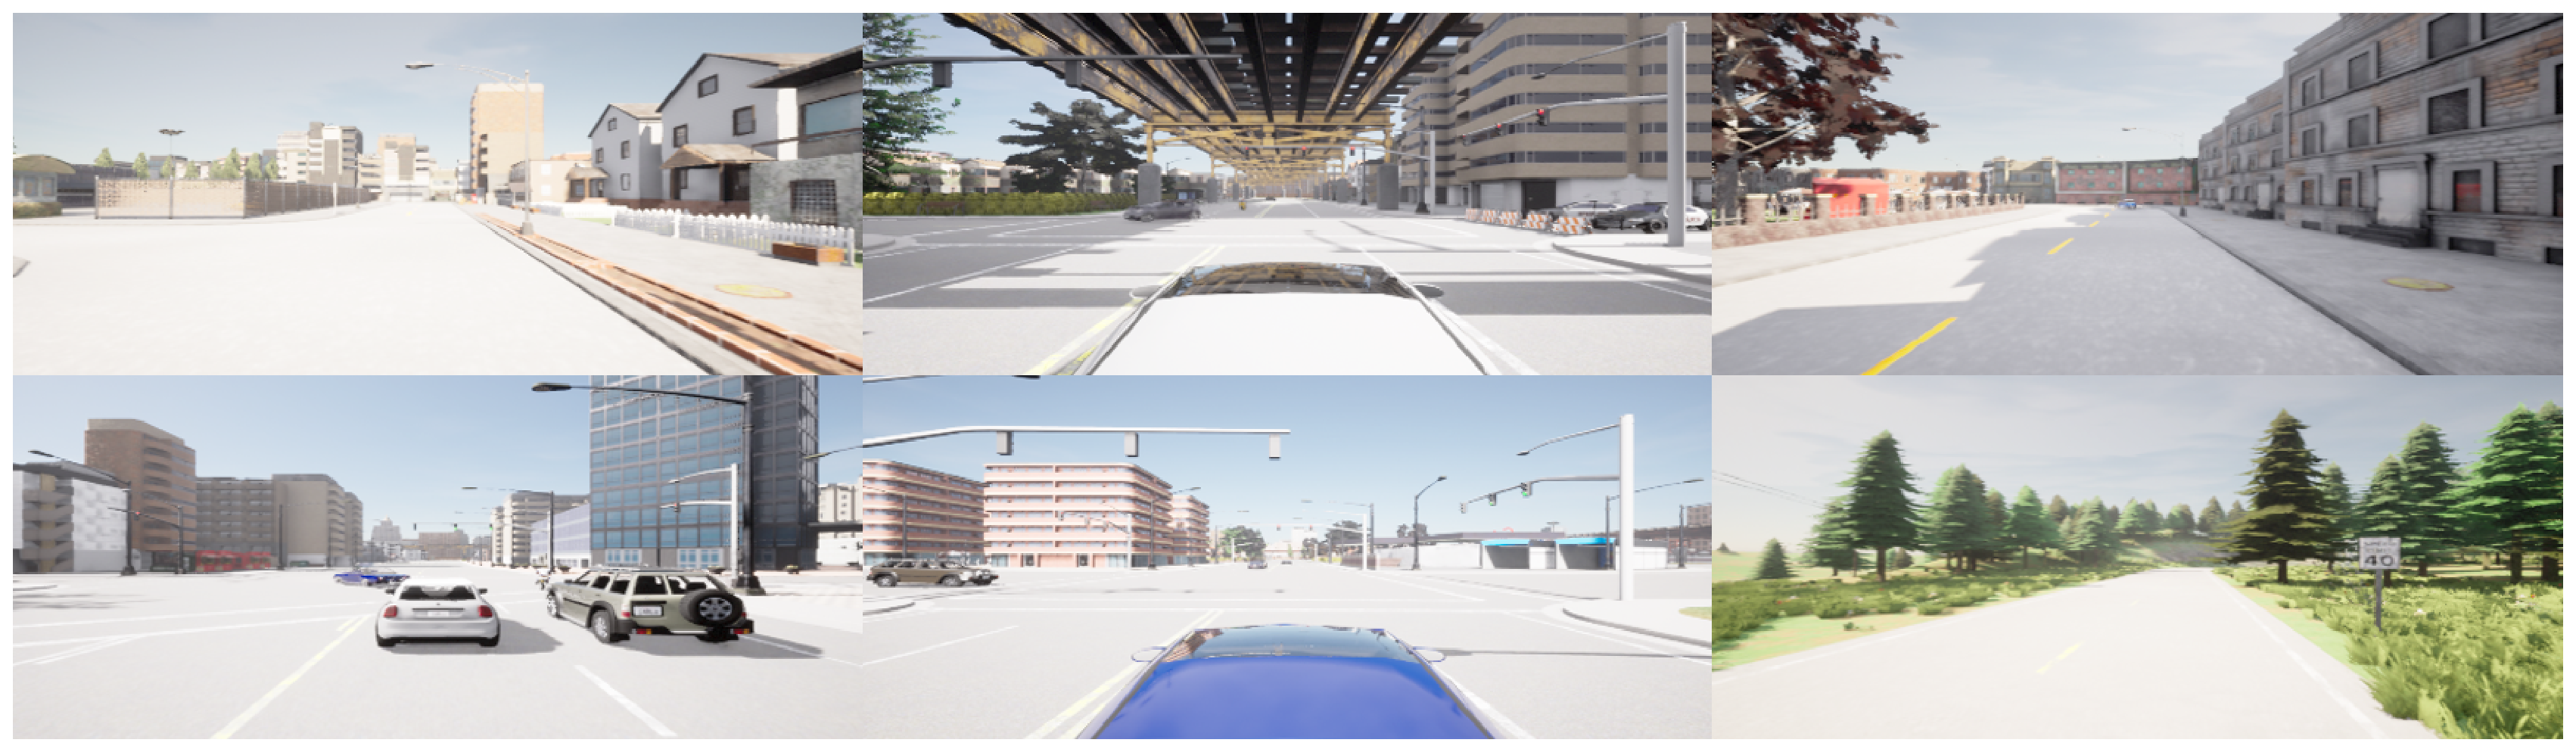
\includegraphics[width=0.9\linewidth]{img/evaluation/CARLA_ex.eps}
  \caption{Examples in CARLA}
  \label{ex_CARLA} 
\end{figure}
\begin{table}[t]
  \centering
  \caption{MAE [m] in CARLA}
  \label{result_MAE_CARLA}
  \begin{tabular}{c|cccc}
      \toprule
      Method                                       & Vehicle            & Person                   \\ \midrule
      PMOD-Net\cite{3}                             & 1.19          & 3.01                 \\ \midrule
      NDDepth\cite{1}                                   & 4.08          & 3.57                 \\ \midrule
      MIMDepth\cite{2}                                    & 3.63          & 3.13                 \\ \midrule
      PMOD-NetD (NDDepth\cite{1})                                  & 1.12          & 2.52                 \\ \midrule
      PMOD-NetD (MIMDepth\cite{2})                                   & $\bm{1.09}$          & $\bm{2.39}$                 \\ \bottomrule
      \end{tabular}
\end{table}
\begin{table}[t]
  \centering
  \caption{MAE [m] in KITTI-360}
  \label{result_MAE_KITTI-360}
  \begin{tabular}{c|cccc}
      \toprule
      Method                                       & Vehicle            & Person         \\ \midrule
      PMOD-Net\cite{3}                                      & 2.27         & 4.10        \\ \midrule
      NDDepth\cite{1}                                            & 4.00         & 4.91        \\ \midrule
      MIMDepth\cite{2}                                             & 4.00         & 4.98        \\ \midrule
      PMOD-NetD (NDDepth\cite{1})                                           & 1.99         & 3.29        \\ \midrule
      PMOD-NetD (MIMDepth\cite{2})                                            & $\bm{1.97}$         & $\bm{3.25}$        \\ \bottomrule
      \end{tabular}
\end{table}
\begin{table}[t]
  \centering
  \caption{{ME [m] in CARLA}}
  \label{result_ME_CARLA}
  \begin{tabular}{c|cc|cc}
      \toprule
      \multirow{2}{*}{Method}  & \multicolumn{2}{c}{Vehicle} & \multicolumn{2}{c}{Person} \\ \cmidrule{2-5} 
                                             & ME+            & ME-          & ME+           & ME-         \\ \midrule
      PMOD-Net\cite{3}                             & 0.571          & -0.423         & 2.52         & -1.76        \\ \midrule
      NDDepth\cite{1}                                   & 2.88          & -2.79         & 2.30          & -5.51        \\ \midrule
      MIMDepth\cite{2}                                    & 2.68          & -1.96         & 1.99          & -5.16        \\ \midrule
      PMOD-NetD                                  & \multirow{2}{*}{0.544}          & \multirow{2}{*}{-0.450}         & \multirow{2}{*}{2.05}          & \multirow{2}{*}{-1.26}        \\ 
      (NDDepth\cite{1})                        &                                  &                                  &                                  &                                 \\ \midrule
      PMOD-NetD                                   & \multirow{2}{*}{$\bm{0.479}$}          & \multirow{2}{*}{$\bm{-0.382}$}         & \multirow{2}{*}{$\bm{1.95}$}          & \multirow{2}{*}{$\bm{-1.23}$}        \\
      (MIMDepth\cite{2})&                                  &                                  &                                  &                                 \\ \bottomrule
    \end{tabular}
\end{table}
\begin{table}[t]
  \centering
  \caption{ME [m] in KITTI-360}
  \label{result_ME_KITTI-360}
  \begin{tabular}{c|cc|cc}
    \toprule
    \multirow{2}{*}{Method}  & \multicolumn{2}{c}{Vehicle} & \multicolumn{2}{c}{Person} \\ \cmidrule{2-5} 
                                           & ME+            & ME-          & ME+           & ME-         \\ \midrule
    PMOD-Net\cite{3}                             & 0.637         & -0.857         & 2.05         & -1.34        \\ \midrule
    NDDepth\cite{1}                                   & 1.40         & -1.27         & 2.02         & -2.76        \\ \midrule
    MIMDepth\cite{2}                                    & 1.43         & -1.26         & 2.09         & -2.78        \\ \midrule
    PMOD-NetD                                  & \multirow{2}{*}{$\bm{0.397}$}          & \multirow{2}{*}{-0.766}         & \multirow{2}{*}{1.02}          & \multirow{2}{*}{-1.38}        \\ 
    (NDDepth\cite{1})                        &                                  &                                  &                                  &                                 \\ \midrule
    PMOD-NetD                                   & \multirow{2}{*}{0.414}          & \multirow{2}{*}{$\bm{-0.751}$}         & \multirow{2}{*}{$\bm{0.942}$}          & \multirow{2}{*}{$\bm{-1.29}$}        \\
    (MIMDepth\cite{2})&                                  &                                  &                                  &                                 \\ \bottomrule
  \end{tabular}
\end{table}
% \begin{table}[t]
%   \centering
%   \caption{ME [m]}
%   \label{result_ME}
%   \begin{tabular}{cc|cc|cc}
%       \toprule
%       \multirow{2}{*}{Method} & \multirow{2}{*}{Class} & \multicolumn{2}{c}{CARLA} & \multicolumn{2}{c}{KITTI-360} \\ \cmidrule{3-6} 
%                          &                    & ME+            & ME-          & ME+           & ME-         \\ \midrule
%       \multirow{2}{*}{PMOD-Net\cite{3}}                  & Vehicle           & 0.571          & -0.423         & 0.637         & -0.857        \\
%                         & Person                  & 2.52          & -1.76         & 2.05         & -1.34        \\ \midrule
%       \multirow{2}{*}{NDDepth\cite{1}}                 & Vehicle                  & 2.88          & -2.79         & 1.40         & -1.27        \\
%                         & Person                  & 2.30          & -5.51         & 2.02         & -2.76        \\ \midrule
%       \multirow{2}{*}{MIMDepth\cite{2}}                  & Vehicle                  & 2.68          & -1.96         & 1.43         & -1.26        \\
%                         & Person                 & 1.99          & -5.16         & 2.09         & -2.78        \\ \midrule
%       \multirow{2}{*}{D}                 & Vehicle                 & 0.544          & -0.450         & $\bm{0.397}$         & -0.766        \\
%                         & Person                 & 2.05          & -1.26         & 1.02         & -1.38        \\ \midrule
%       \multirow{2}{*}{E}                  & Vehicle                 & $\bm{0.479}$          & $\bm{-0.382}$         & 0.414         & $\bm{-0.751}$        \\
%                         & Person                 & $\bm{1.95}$          & $\bm{-1.23}$         & $\bm{0.942}$         & $\bm{-1.29}$        \\ \bottomrule
%       \end{tabular}
% \end{table}
\subsection{実験結果と考察}
各データセットにおける結果を\reftable{result_MAE_CARLA}，\reftable{result_MAE_KITTI-360}，\reftable{result_ME_CARLA}，\reftable{result_ME_KITTI-360}に示す．\reffig{result_CARLA}，\reffig{result_KITTI-360}は，
Segmentation結果と推定距離画像から作成した点群の鳥瞰図である．
\begin{figure}[t]
  \centering
  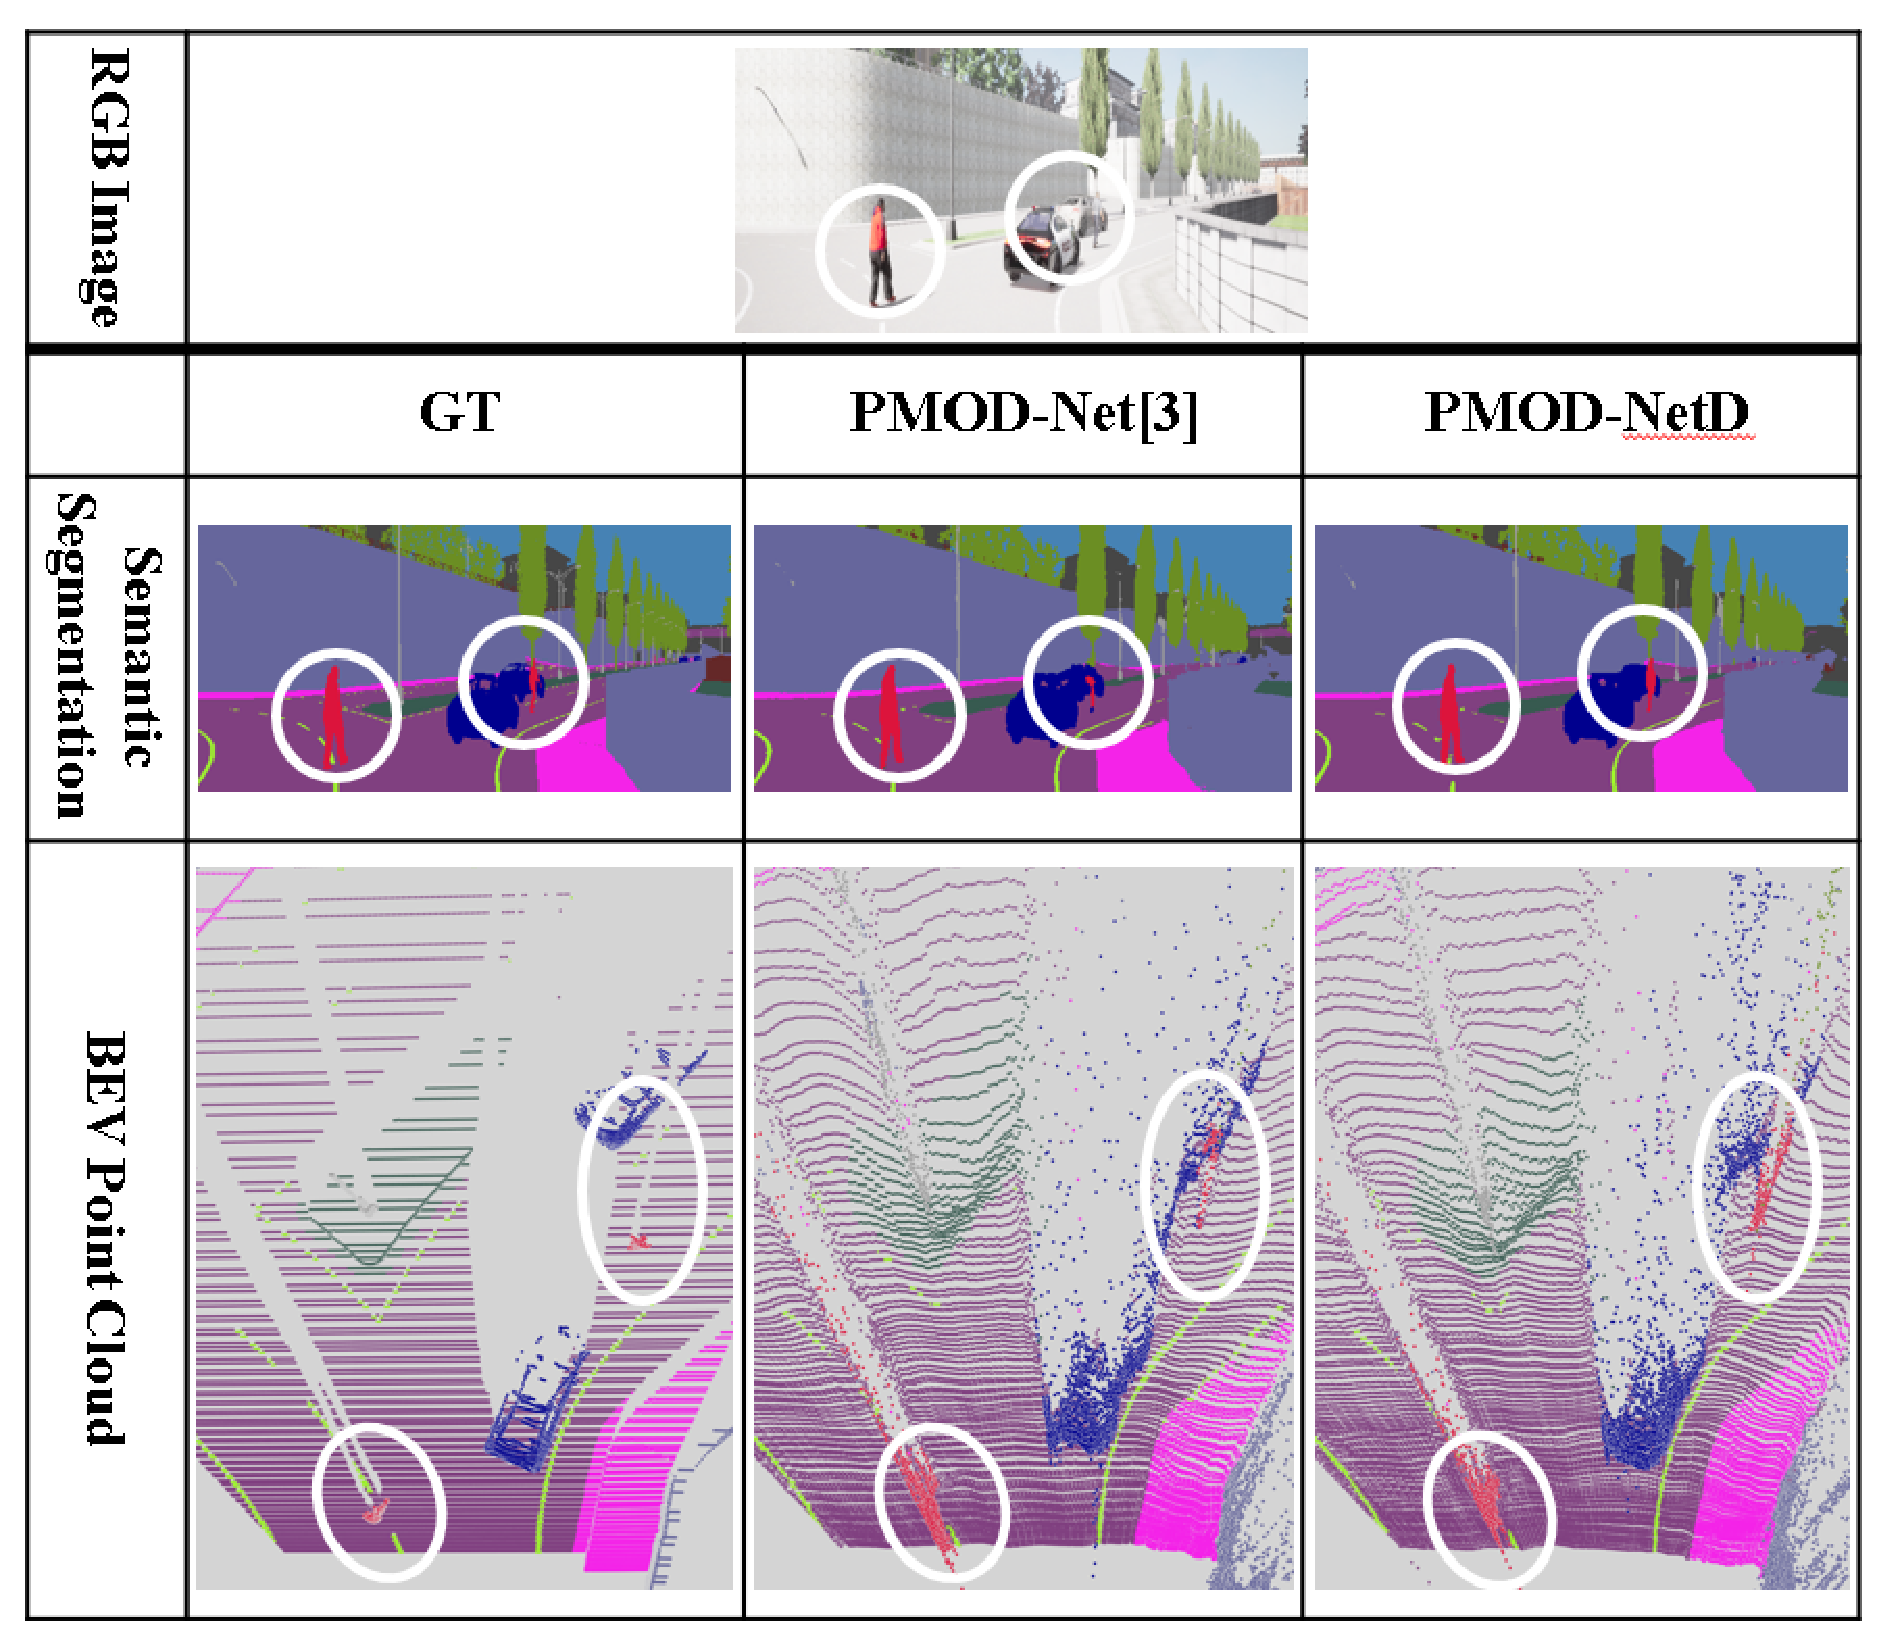
\includegraphics[width=0.935\linewidth]{img/evaluation/result_CARLA.eps}
  \caption{Experimental results in CARLA}
  \label{result_CARLA} 
\end{figure}
\begin{figure}[t]
  \centering
  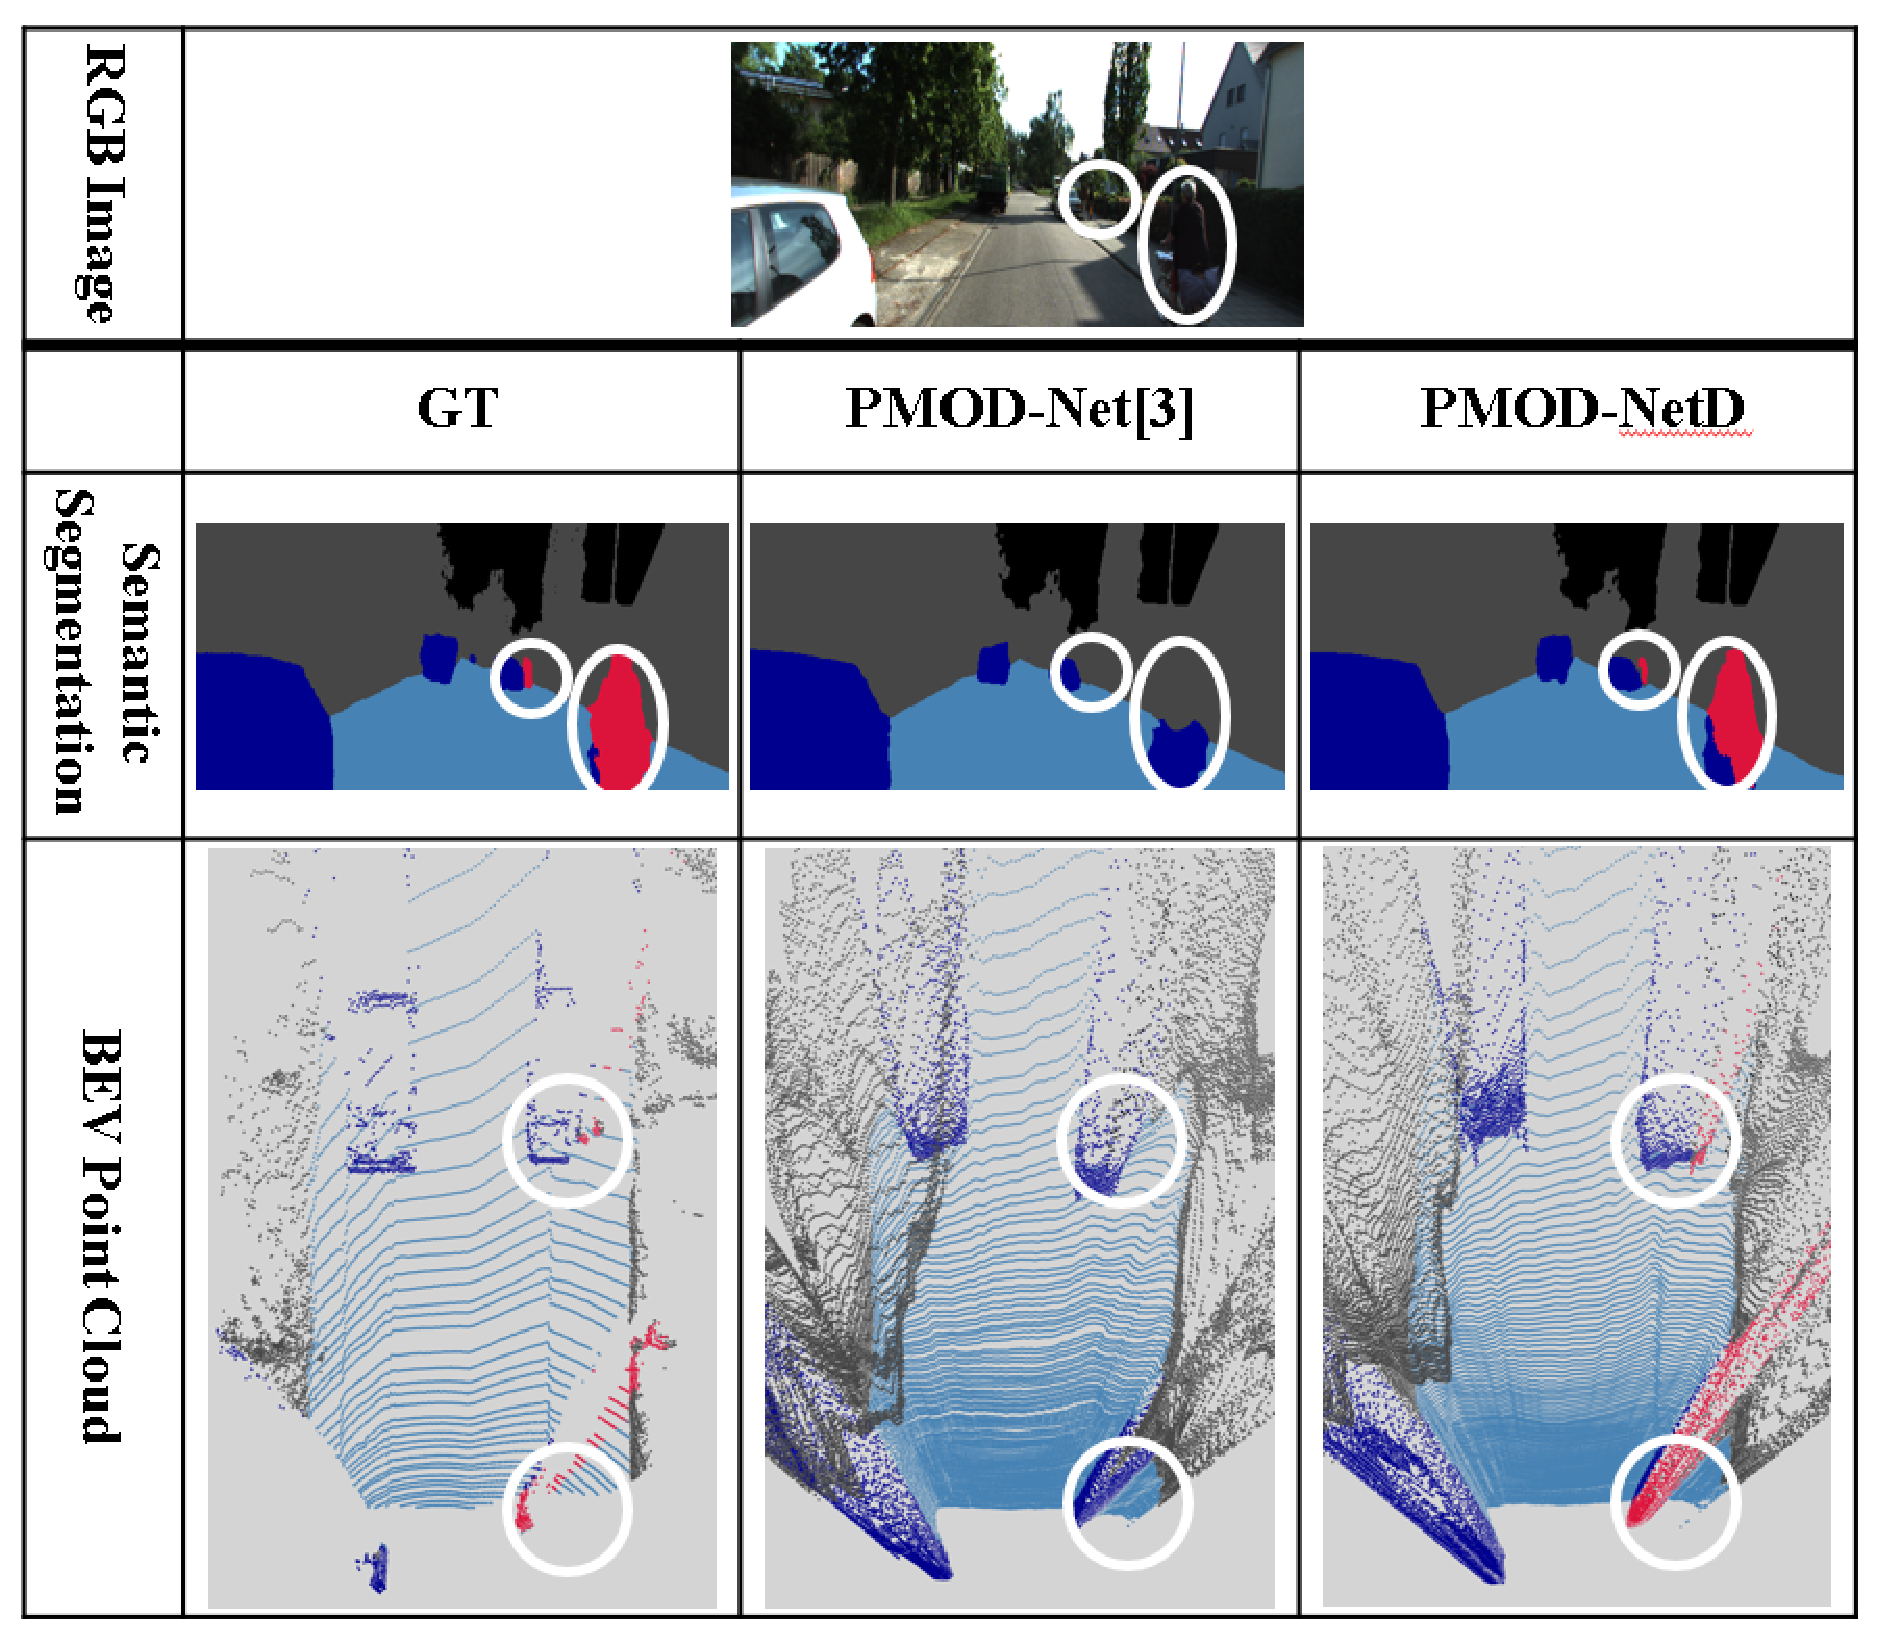
\includegraphics[width=0.935\linewidth]{img/evaluation/result_KITTI-360.eps}
  \caption{Experimental results in KITTI-360}
  \label{result_KITTI-360} 
\end{figure}

\reftable{result_MAE_CARLA}，\reftable{result_MAE_KITTI-360}の実験結果からPMOD-NetDはPMOD-Netよりも精度が向上していることが
わかった．新たに単眼深度画像を導入したことで，動的障害物の
距離推定精度向上に影響を与えたと考える．従来の PMOD-Net
では移動ロボットを利用した低速自動運転において，約2.8m
の間隔で配置された障害物の回避を実現している\cite{3}．本手法はPMOD-Netより精度向上
したため，さらに狭い間隔で障害物が配置された複雑な環境での自動運転に貢献できると
考えられる．

さらに\reffig{result_KITTI-360}のSegmentation結果
を見るとPMOD-Netでは検出できていない人が検出できていることもわかる．
単眼深度推定で障害物の境界を明確にすることは，セグメンテーション結果
にも有用であることが考察された．またNDDepthを用いた場合もMIMDepthを
用いた場合も，元の単眼深度推定結果よりもPMOD-NetDの方が高精度となった．
精度が良いMIMDepthを基にしたPMOD-NetDの方が，より精度が高い．したがって
今後高精度な単眼深度推定が開発された際に，PMOD-NetDに応用することで，
さらなる高精度化が期待できる．

しかし鳥瞰図を見ると，障害物の後方への距離推定誤差がまだ大きいことがわかる．
距離的に遠方にある背景の影響が強いため，障害物の境界を
強調して学習する損失などの導入が必要である．

\reftable{result_ME_CARLA}，\reftable{result_ME_KITTI-360}の実験結果から，本提案手法では，推定位置が正解より手前か奥かといっ
た傾向がデータセットごとに異なることがわかる．データセット内に含まれる物体の距離
の分布によって傾向が異なると考えられるため，手前に推定させたい場合は，データセット
に含まれる物体までの距離を全体的に短くするなど，学習させる距離の分布を調整するこ
とは重要である．


\section{まとめ}
本研究では，単眼カメラでの距離推定を目的とし，三次元
地図上に存在しない動的障害物の検出精度を向上させるこ
とを目指した．単眼深度推定手法と三次元地図を統合し，動
的障害物の距離を推定するPMOD-NetDを開発した．PMOD-NetDは，公開データセットKITTI-360において人の距離推
定誤差平均は3.25[m]となり，
従来のPMOD-Netより0.85[m]
減少することを確認した．また，KITTIデータセットにおい
て高精度なNDDepthやMIMDepthといった複数の深度推定法
の精度を向上させられる汎用性を持つことが確認された．
今後は，動的障害物の境界に特化した新たな損失を追加し，
障害物回避実験を実施する．
\small
\begin{thebibliography}{14}
    \bibitem{1}
    S. Shao, et al, NDDepth: Normal-distance assisted monocular depth estimation and completion, International Conference on Computer Vision, 2023. 
    \bibitem{2}
    Z. Xie, et al, Revealing the dark secrets of masked image modeling, Computing Research Repository, 2022.
    \bibitem{3}
    J. Shikishima, et al, PMOD-Net: point-cloud-map-based metric scale obstacle detection by using a monocular camera, Advanced Robotics, 2022.
    \bibitem{4}
    K. Deng, et al, Depth-supervised nerf: Fewer views and faster training for free, Computer Vision and Pattern Recognition, 2022.
    \bibitem{5}
    B. Zhou, et al, Does computer vision matter for action? , Science Robotics, 2019.
    \bibitem{6}
    D. Park, et al, Is pseudo-lidar needed for monocular 3d object detection?, International Conference on Computer Vision, 2021.
    \bibitem{7}
    A. Geiger, et al, Are we ready for autonomous driving? The kitti vision benchmark suite, Computer Vision and Pattern Recognition Conference, 2012
    \bibitem{8}
    N. Silberman, et al, Indoor segmentation and support inference from rgbd images, European Conference on Computer Vision, 2012.
    \bibitem{9}
    V. A. Sindagi, et al, MVX-Net: Multimodal voxelnet for 3D object detection, International Conference on Robotics and Automation, 2019.
    \bibitem{10}
    H. Wu, et al, Virtual Sparse Convolution for Multimodal 3D Object Detection, Computer Vision and Pattern Recognition Conference, 2023.
    \bibitem{11}
    Z. Chen, et al, A Strip Adjustment Method of UAV-Borne LiDAR Point Cloud Based on DEM Features for Mountainous Area, the 6th National Lidar Conference , 2021.
    \bibitem{12}
    L. Yang, et al, Efficient plane extraction using normal estimation and RANSAC from 3D point cloud, Computer Standards \& Interfaces, 2022.
    \bibitem{13}
    A. Dosovitskiy, et al, CARLA: An Open Urban DrivingSimulator, Conference on Robot Learning, 2017.
    \bibitem{14}
    Y. Liao, et al, KITTI-360: A novel dataset and benchmarksfor urban scene understanding in 2d and 3d, Transactions on Pattern Analysis and Machine Intelligence, 2022.
\end{thebibliography}

% \section{はじめに}
自動運転における事故防止を目的とした障害物回避のた
めに障害物を認識し，自車から障害物までの距離を推定す
る必要がある．自動運転車でよく用いられる距離センサは
LiDAR(Light Detection and Ranging)である．しかし，
LiDAR は高価であり，メンテナンスに手間がかかる．そこ
で本研究では安価な単眼カメラによる障害物検出を目的と
する．

単眼カメラによる深度推定法として NDDepth\cite{1}や
MIMDepth\cite{2}などがある．しかし，これらの手法は単眼
カメラ画像のみで深度を推定するため，推定結果を実距離
にするスケールパラメータが不定であり，正確な距離を推
定することは困難である．以降，スケールが特定された深
度を距離，スケールが特定されていない深度を単に深度と
して区別して使用する．

単眼カメラ画像に加えて，自動運転用に作成された三次
元地図\reffig{3Dmap}を入力に用いることで，障害物までの距
離を推定できるPMOD-Net\cite{3}がある．正確な距離情報を
持つ三次元地図により，PMOD-Net は単眼カメラ画像で正
確な距離を推定しつつ障害物検出が可能である．

PMOD-Net は，三次元地図と単眼カメラ画像を入力とし
て，Semantic Segmentation と距離推定をマルチタスク
に行う．Semantic Segmentation で三次元地図上に存在
しない人や車などの動的障害物を検出することにより，距
離推定タスクで動的障害物の距離も推定可能にした．しか
し，三次元地図は動的障害物の距離情報を持たないため，
地図上に存在する障害物の距離推定精度に比べて，動的障
害物の距離推定精度は低い．そこで本研究は，単眼カメラ
を用いて，三次元地図上に存在しない動的障害物までの距
離を推定するという課題に取り組む．
\begin{figure}[t]
  \centering
  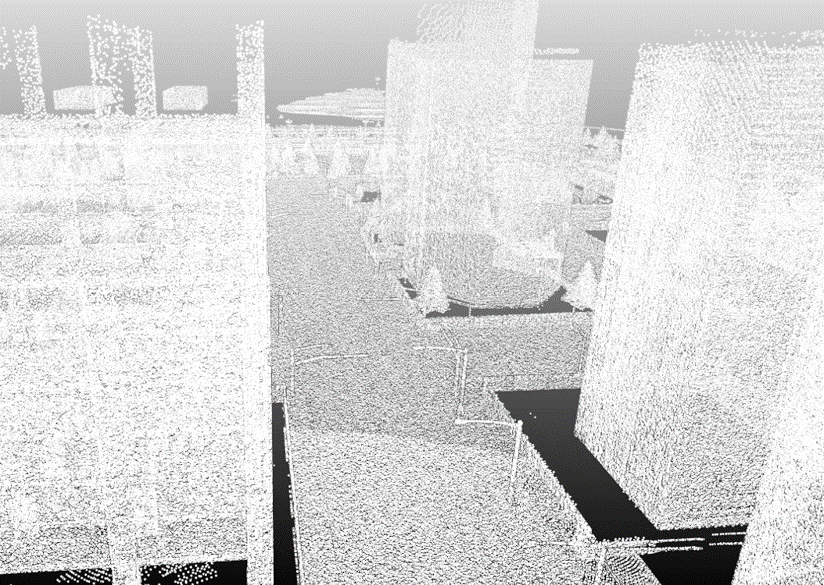
\includegraphics[width=0.95\linewidth]{img/intro/3Dmap.png}
  \caption{3D map}
  \label{3Dmap} 
\end{figure}

課題を解決するために，地図を使用する距離推定と地図
を使用しない深度推定の相補的な関係に着目した．三次元
地図を利用するPMOD-Net は距離を推定できるが，地図
の影響で動的障害物に対する距離推定精度は低い．地図を
使用しないNDDepth やMIMDepth は深度しか推定できないが，
動的障害物も含め，現在画像内にある全物体の相
対的な深度を精度よく推定できる．そこで，地図を使用し
ない単眼深度
推定法の出力を PMOD-Net へ入力する新手法 PMOD-
NetD（PMOD-Net with Depth）を開発する．三次元地
図という過去の距離情報と，単眼深度推定からの現在の深
度情報を統合し，単眼カメラによる高精度な障害物検出を
実現する．

本研究の学術的貢献は以下である．
\begin{enumerate}[1.]
  \begin{figure*}[t]
      \centering
      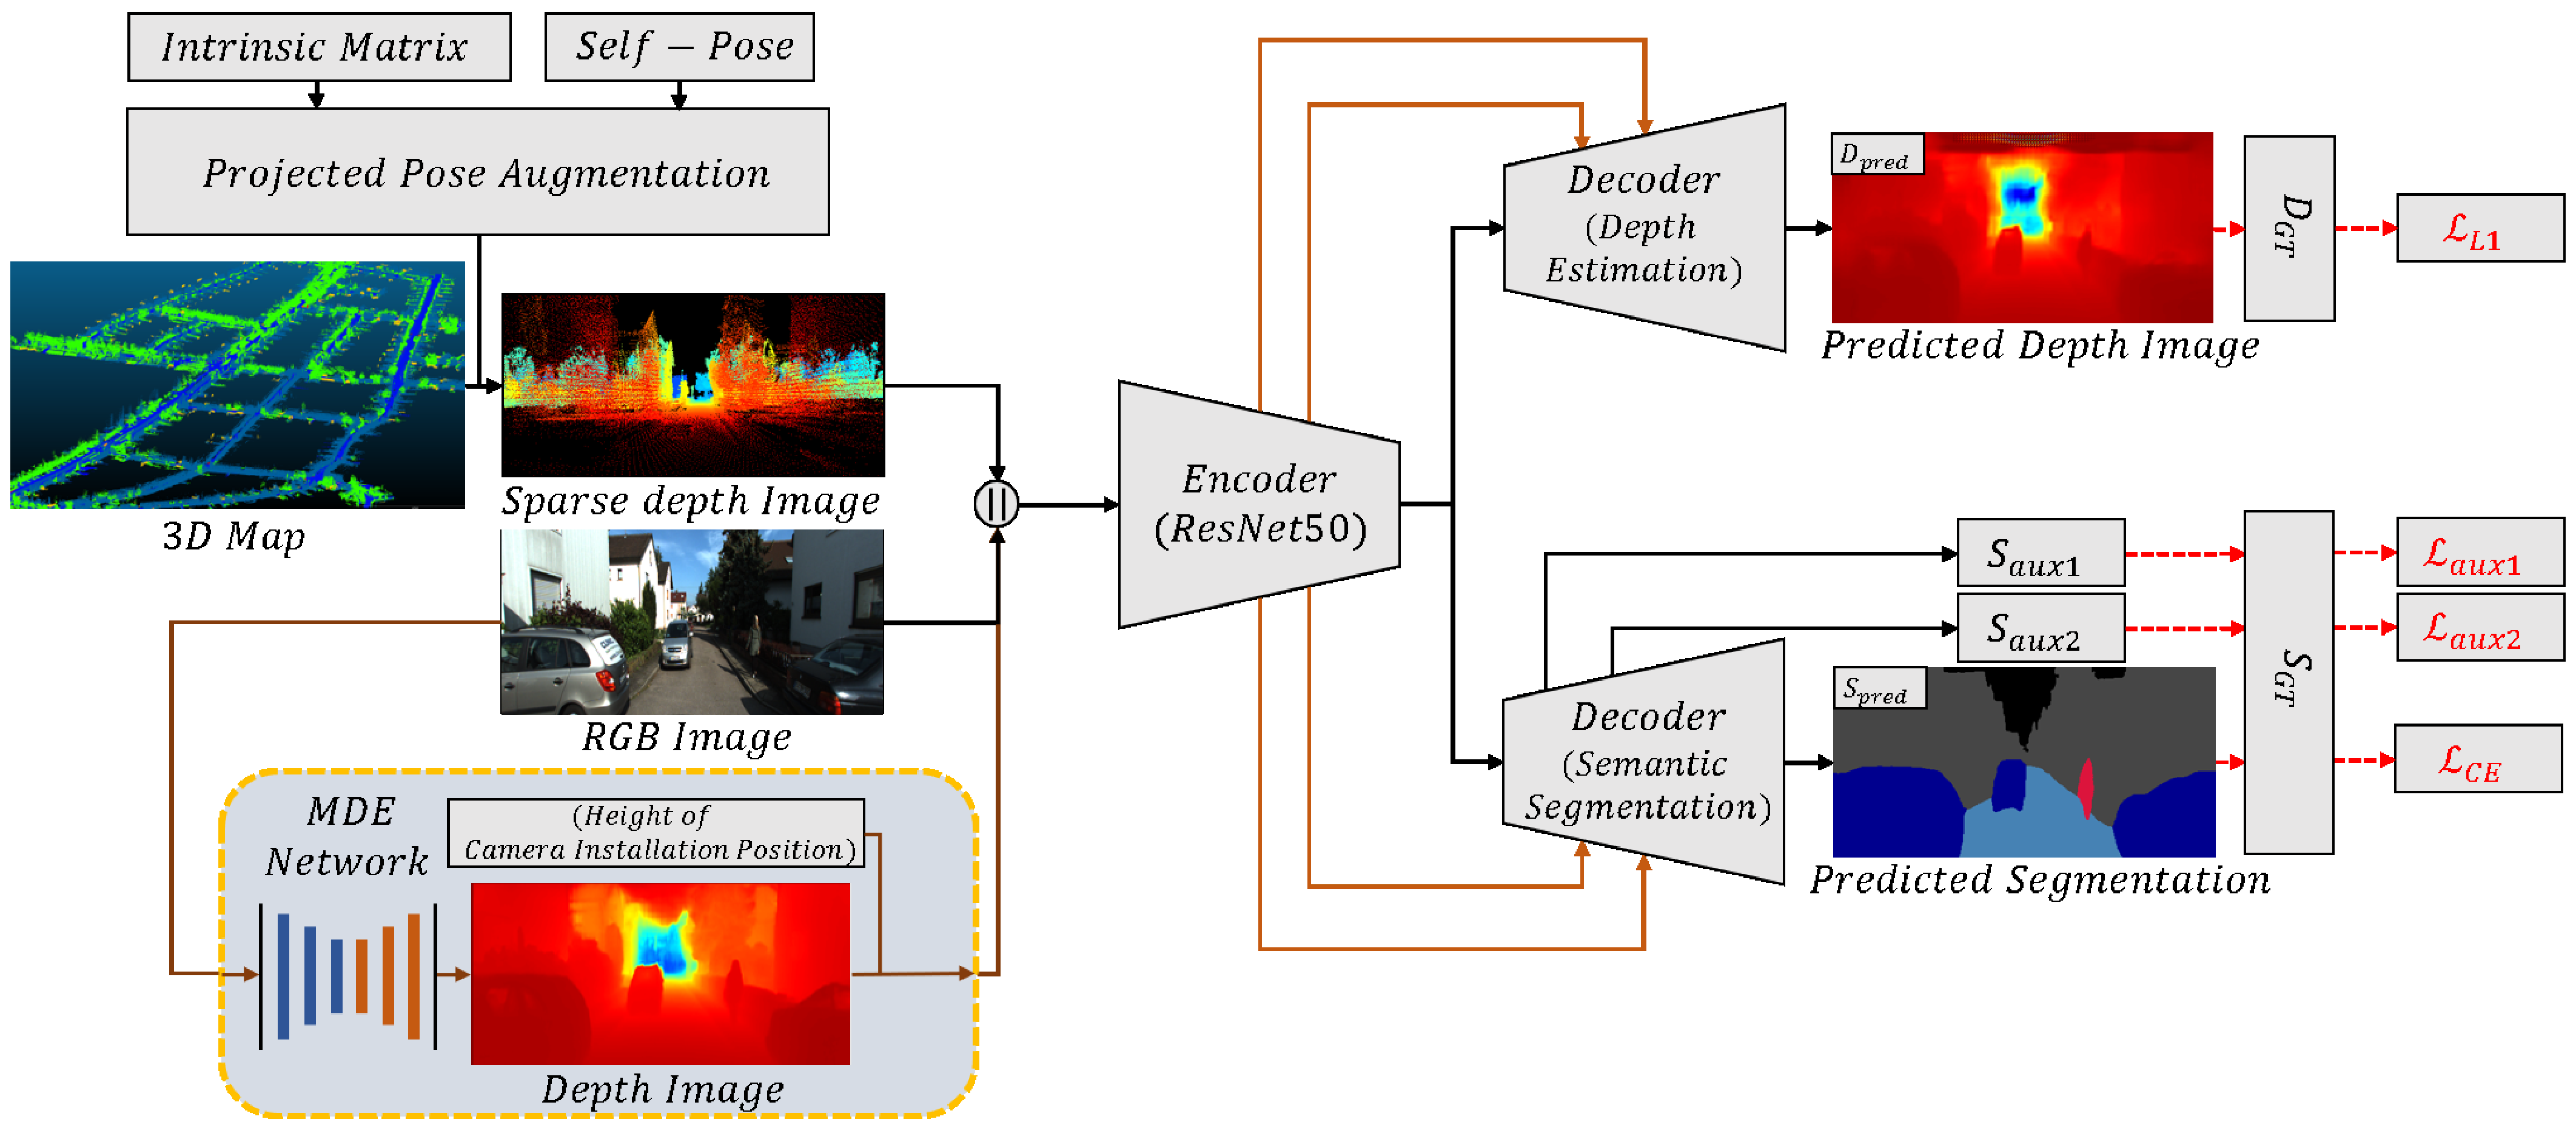
\includegraphics[width=0.95\linewidth]{img/method/network_architecture.eps}
      \caption{Network architecture of PMOD-NetD}
      \label{networkarchitecture} 
  \end{figure*}
  \item 三次元地図と単眼カメラを用いて三次元的に障害物検出を行う世界初のニューラルネットワークであるPMOD-Net を高精度化する新手法を開発した．
  \item スケールが不定であるため手法単体で扱うことが困難な単眼深度推定結果に対して三次元地図によるスケール調整が有効であることを示した．
  \item KITTI ベンチマークにおいて高順位の複数の単眼深度推定法に対して性能を高められることを確認し，手法を問わずに高精度化できる汎用性を示した．
\end{enumerate}
% \section{関連研究}

\subsection{単眼深度推定}
単眼深度推定は3Dモデリング\cite{4}，ロボット工学\cite{5}，自
動運転\cite{6}などに応用され，盛んに研究されている．これら
の手法はスケールが類似した大量のデータセットで学習・
テストを行うことで，学習時と同一の環境であれば距離推
定可能である．NDDepth\cite{1}やMIMDepth\cite{2}はKITTI\cite{7}
，NYUDepth-v2\cite{8}の2 種類のデータセットにおいて高い
精度を示した．しかし，学習した環境と異なる環境では，
深度から距離へと変換するためのスケールの推定が必要と
なる．したがってスケールの推定精度によっては精度が大
きく低下する可能性がある．
\subsection{距離補完}
入力にLiDAR 点群とカメラ画像を用いてLiDAR 点群を
補完し，密な距離画像を生成する距離補完手法も多く研究
されている\cite{9}\cite{10}．三次元地図点群を疑似的なLiDAR 点
群とみなすことで，距離画像の生成が可能である．しかし，
カメラ画像とLiDAR 点群は同時刻に取得されることが前提
の手法であり，画像内の物体とLiDAR 点群は一致している
ことが望まれる．そのため三次元地図上に存在しない車や
人などの動的障害物の距離推定においてPMOD-Net\cite{3}と
同等の精度を得るのは困難である．
\subsection{PMOD-Net}
PMOD-Net\cite{3}は地図から作成した疎な距離画像とカメ
ラ画像を入力として，Semantic Segmentation と距離推
定を行う世界初のニューラルネットワークである．
Semantic Segmentation と距離推定をマルチタスクに行
うことで三次元地図上に存在しない動的障害物を含めた三
次元障害物検出を可能にした．疎な距離画像は，自己位置
推定結果をもとに三次元地図点群を画像平面に投影するこ
とで取得する．自己位置はGPS やIMU，オドメトリ，カ
メラなどで取得した値を利用する．
\subsection{本研究の位置づけ}
PMOD-Netは，単眼カメラで障害物までの正確な距離を
計測できる利点がある．さらに実際に移動ロボットで障害
物回避にも成功しているため，本研究でもベース手法とし
て使用する．本研究は，単眼カメラのみでの代表的な距離
推定手法である単眼深度推定法とPMOD-Net\cite{3}を利用す
る．しかし，双方の相補的な関係に着目し，欠点を単一
ネットワーク内で同時に解決する新手法を開発したという
点で従来とは大きく異なる．

また本研究は，開発スピードが速い単眼深度推定分野に
おいて，深度推定法そのものを開発するものではない．地
図を利用することで，深度推定法によらずに距離推定を高
精度化する手法を開発している点も，従来とは大きく異な
る．さらに従来の学習を必要としないスケー
ル調整に加えて，学習ベースでスケールを調整するという新規性があり，より高精度な距離
推定を可能にしている．




% \section{提案手法}

新たに開発したPMOD-NetDの構造を\reffig{networkarchitecture}に示す．
カメラ画像から深度画像を作成し，スケール調整を行う．
ここで深度画像の作成には単眼深度推定用のニューラル
ネットワーク (Monocular Depth Estimation:MDE Network) を用いる．本研究の評価実験ではMDE
Networkとして，NDDepth\cite{1}やMIMDepth\cite{2}を用い
た．またMDE Networkが学習した環境であれば，スケー
ル調整は不要であるため，行わない．学習していない環境
であれば，スケールの調整を行う．

スケールの調整方法として，地面の高さを用いる手法
\cite{11}を利用する．地面を利用したスケール調整方法の手順
を以下に示す．
\begin{enumerate}[1.]
    \item RANSAC\cite{12}で平面推定を行い，単眼深度推定の出
    力から地面点群を抽出する．
    \item 事前に取得したカメラの高さ$z$を用いて式(\ref{Scale_S})でスケール
    $S$を算出する．ここで$P_c^{i}$と$N$はそれぞれ，単眼深度推定か
    ら得られた地面点群における点$i$の高さと点群数を示す．
    \begin{equation}
        \label{Scale_S}
        S= \frac{z}{\frac{1}{N}{}\sum_{i=1}^{N}P_c^{i}} 
    \end{equation}
\end{enumerate}

ここで取得した$S$と深度画像$I_o$からスケール調整した距離画
像$I_D$を式(\ref{metric_Id})のように取得する．
\begin{equation}
    \label{metric_Id}
    I_D=S*I_o
\end{equation}

カメラ画像と疎な距離画像，距離画像$I_D$をチャンネル方向に
結合し，PMOD-NetDの入力とする．常に絶対的な距離情報をも
つ三次元地図と入力段階で結合することで前述した欠点を補い
つつ学習を進めることができる．

また距離画像$I_D$は，任意のMDE Networkから作成可能であり，
精度が良い手法であるほど，最終的な精度を高めることができ
る．そのため，PMOD-NetとMDE Networkどちらの開発が進んで
も，精度向上に寄与することができる．
% \section{評価実験}
\subsection{実験設定}
提案手法の有効性を確認するために，以下 2 つのデータ
セットで評価実験を行った．
\begin{enumerate}[1.]
  \item シミュレーションデータセット (CARLA\cite{13})
  \item 公開データ (KITTI-360 データセット\cite{14})
\end{enumerate}

どちらのデータセットにおいても，PMOD-NetDと，以下3つの手法と比較する．
\begin{enumerate}[1.]
  \item PMOD-Net\cite{3}
  \item NDDepth\cite{1}
  \item MIMDepth\cite{2}
\end{enumerate}

NDDepthとMIMDepthはKITTIデータセットで高い精度を
出しており，事前学習済みのモデルも公開されているため，
比較手法として用いることにした．学習済みのモデルが公
開されているため，KITTI-360データセットではスケール調
整不要で距離精度の比較が可能である．CARLAで使用する場
合は式(\ref{metric_Id})のようにスケール調整した結果で比較する．ここ
では2.0[m]の位置にカメラを設置した．
\subsection{使用データセット}
シミュレーションデータセットは，自動運転研究用シミュレ
ータである CARLA\cite{13}を用いて作成した．CARLAには特徴の異
なる7種類のマップがあり，マップごとにランダムに配置され
た人や車を含むデータセットを作成した．学習データには各マ
ップから600枚ずつ，合計4200枚を使用し，テストには各マッ
プから学習に使用していない1840 枚ずつ，合計12880 枚を用
いた．\reffig{ex_CARLA}に学習および評価に使用した画像例を示す．三次
元地図の投影にはシミュレータが出力するカメラ位置を用いた．
公開データセットとしてKITTI-360\cite{14}を使用した．ドイツ
郊外を撮影した大規模な車載センサデータセットであり，9つ
のシーケンスを提供している．本実験ではデータ数が少ないシ
ーケンス03を除いた8シーケンスの三次元地図と左カメラ画
像を使用した．学習データには各シーケンスから500枚ずつ，
合計4000枚を使用し，テストには学習に使用していないデー
タをすべて用いた．テスト時にはKITTI-360が提供している自
己位置誤差を含んだ慣性航法システムのデータを使用し，実際
の位置誤差を想定した実験を行った．

\subsection{評価指標}
評価は画像中の動的障害物に対して行う．本実験では人と車
を動的障害物とした．距離推定の評価指標には，距離誤差平均
を示すMAEを用いる．MAEは式(\ref{MAE})で計算する．$n$は評価対象の
領域を示す画素数であり,$i$は画素位置である．$D_P$は各手法が推
定した距離画像，$D_{GT}$は正解の距離画像である．ともにカメラか
ら各物体までの距離を示す．また方向性のあ
る誤差を評価するため，式(\ref{MAE})において絶対値内の値が正の場合と負の場合だけを評価した
値をそれぞれ ME+，ME-として分けて評価する．
\begin{equation}
  \label{MAE}
  MAE= \frac{1}{n}{}\sum_{i=1}^{n}|D_P(i)-D_{GT}(i)|
\end{equation}
\begin{figure}[t]
  \centering
  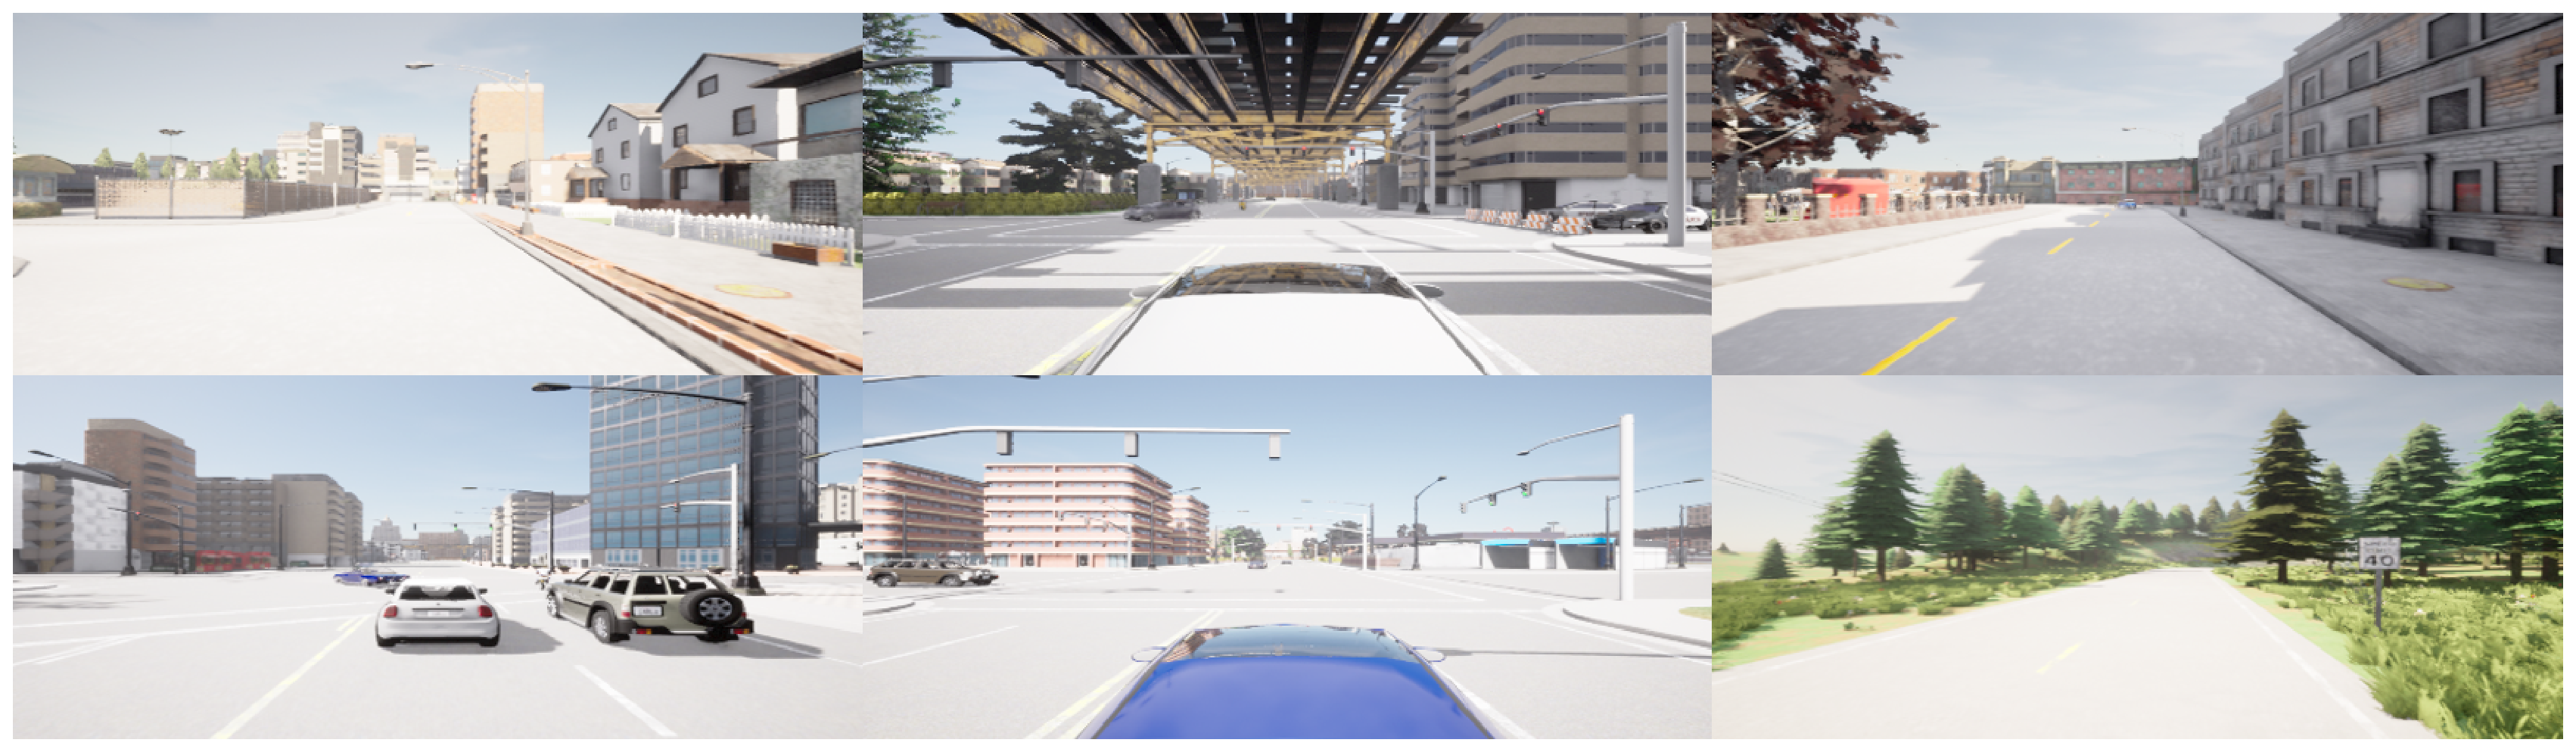
\includegraphics[width=0.9\linewidth]{img/evaluation/CARLA_ex.eps}
  \caption{Examples in CARLA}
  \label{ex_CARLA} 
\end{figure}
\begin{table}[t]
  \centering
  \caption{MAE [m] in CARLA}
  \label{result_MAE_CARLA}
  \begin{tabular}{c|cccc}
      \toprule
      Method                                       & Vehicle            & Person                   \\ \midrule
      PMOD-Net\cite{3}                             & 1.19          & 3.01                 \\ \midrule
      NDDepth\cite{1}                                   & 4.08          & 3.57                 \\ \midrule
      MIMDepth\cite{2}                                    & 3.63          & 3.13                 \\ \midrule
      PMOD-NetD (NDDepth\cite{1})                                  & 1.12          & 2.52                 \\ \midrule
      PMOD-NetD (MIMDepth\cite{2})                                   & $\bm{1.09}$          & $\bm{2.39}$                 \\ \bottomrule
      \end{tabular}
\end{table}
\begin{table}[t]
  \centering
  \caption{MAE [m] in KITTI-360}
  \label{result_MAE_KITTI-360}
  \begin{tabular}{c|cccc}
      \toprule
      Method                                       & Vehicle            & Person         \\ \midrule
      PMOD-Net\cite{3}                                      & 2.27         & 4.10        \\ \midrule
      NDDepth\cite{1}                                            & 4.00         & 4.91        \\ \midrule
      MIMDepth\cite{2}                                             & 4.00         & 4.98        \\ \midrule
      PMOD-NetD (NDDepth\cite{1})                                           & 1.99         & 3.29        \\ \midrule
      PMOD-NetD (MIMDepth\cite{2})                                            & $\bm{1.97}$         & $\bm{3.25}$        \\ \bottomrule
      \end{tabular}
\end{table}
\begin{table}[t]
  \centering
  \caption{{ME [m] in CARLA}}
  \label{result_ME_CARLA}
  \begin{tabular}{c|cc|cc}
      \toprule
      \multirow{2}{*}{Method}  & \multicolumn{2}{c}{Vehicle} & \multicolumn{2}{c}{Person} \\ \cmidrule{2-5} 
                                             & ME+            & ME-          & ME+           & ME-         \\ \midrule
      PMOD-Net\cite{3}                             & 0.571          & -0.423         & 2.52         & -1.76        \\ \midrule
      NDDepth\cite{1}                                   & 2.88          & -2.79         & 2.30          & -5.51        \\ \midrule
      MIMDepth\cite{2}                                    & 2.68          & -1.96         & 1.99          & -5.16        \\ \midrule
      PMOD-NetD                                  & \multirow{2}{*}{0.544}          & \multirow{2}{*}{-0.450}         & \multirow{2}{*}{2.05}          & \multirow{2}{*}{-1.26}        \\ 
      (NDDepth\cite{1})                        &                                  &                                  &                                  &                                 \\ \midrule
      PMOD-NetD                                   & \multirow{2}{*}{$\bm{0.479}$}          & \multirow{2}{*}{$\bm{-0.382}$}         & \multirow{2}{*}{$\bm{1.95}$}          & \multirow{2}{*}{$\bm{-1.23}$}        \\
      (MIMDepth\cite{2})&                                  &                                  &                                  &                                 \\ \bottomrule
    \end{tabular}
\end{table}
\begin{table}[t]
  \centering
  \caption{ME [m] in KITTI-360}
  \label{result_ME_KITTI-360}
  \begin{tabular}{c|cc|cc}
    \toprule
    \multirow{2}{*}{Method}  & \multicolumn{2}{c}{Vehicle} & \multicolumn{2}{c}{Person} \\ \cmidrule{2-5} 
                                           & ME+            & ME-          & ME+           & ME-         \\ \midrule
    PMOD-Net\cite{3}                             & 0.637         & -0.857         & 2.05         & -1.34        \\ \midrule
    NDDepth\cite{1}                                   & 1.40         & -1.27         & 2.02         & -2.76        \\ \midrule
    MIMDepth\cite{2}                                    & 1.43         & -1.26         & 2.09         & -2.78        \\ \midrule
    PMOD-NetD                                  & \multirow{2}{*}{$\bm{0.397}$}          & \multirow{2}{*}{-0.766}         & \multirow{2}{*}{1.02}          & \multirow{2}{*}{-1.38}        \\ 
    (NDDepth\cite{1})                        &                                  &                                  &                                  &                                 \\ \midrule
    PMOD-NetD                                   & \multirow{2}{*}{0.414}          & \multirow{2}{*}{$\bm{-0.751}$}         & \multirow{2}{*}{$\bm{0.942}$}          & \multirow{2}{*}{$\bm{-1.29}$}        \\
    (MIMDepth\cite{2})&                                  &                                  &                                  &                                 \\ \bottomrule
  \end{tabular}
\end{table}
% \begin{table}[t]
%   \centering
%   \caption{ME [m]}
%   \label{result_ME}
%   \begin{tabular}{cc|cc|cc}
%       \toprule
%       \multirow{2}{*}{Method} & \multirow{2}{*}{Class} & \multicolumn{2}{c}{CARLA} & \multicolumn{2}{c}{KITTI-360} \\ \cmidrule{3-6} 
%                          &                    & ME+            & ME-          & ME+           & ME-         \\ \midrule
%       \multirow{2}{*}{PMOD-Net\cite{3}}                  & Vehicle           & 0.571          & -0.423         & 0.637         & -0.857        \\
%                         & Person                  & 2.52          & -1.76         & 2.05         & -1.34        \\ \midrule
%       \multirow{2}{*}{NDDepth\cite{1}}                 & Vehicle                  & 2.88          & -2.79         & 1.40         & -1.27        \\
%                         & Person                  & 2.30          & -5.51         & 2.02         & -2.76        \\ \midrule
%       \multirow{2}{*}{MIMDepth\cite{2}}                  & Vehicle                  & 2.68          & -1.96         & 1.43         & -1.26        \\
%                         & Person                 & 1.99          & -5.16         & 2.09         & -2.78        \\ \midrule
%       \multirow{2}{*}{D}                 & Vehicle                 & 0.544          & -0.450         & $\bm{0.397}$         & -0.766        \\
%                         & Person                 & 2.05          & -1.26         & 1.02         & -1.38        \\ \midrule
%       \multirow{2}{*}{E}                  & Vehicle                 & $\bm{0.479}$          & $\bm{-0.382}$         & 0.414         & $\bm{-0.751}$        \\
%                         & Person                 & $\bm{1.95}$          & $\bm{-1.23}$         & $\bm{0.942}$         & $\bm{-1.29}$        \\ \bottomrule
%       \end{tabular}
% \end{table}
\subsection{実験結果と考察}
各データセットにおける結果を\reftable{result_MAE_CARLA}，\reftable{result_MAE_KITTI-360}，\reftable{result_ME_CARLA}，\reftable{result_ME_KITTI-360}に示す．\reffig{result_CARLA}，\reffig{result_KITTI-360}は，
Segmentation結果と推定距離画像から作成した点群の鳥瞰図である．
\begin{figure}[t]
  \centering
  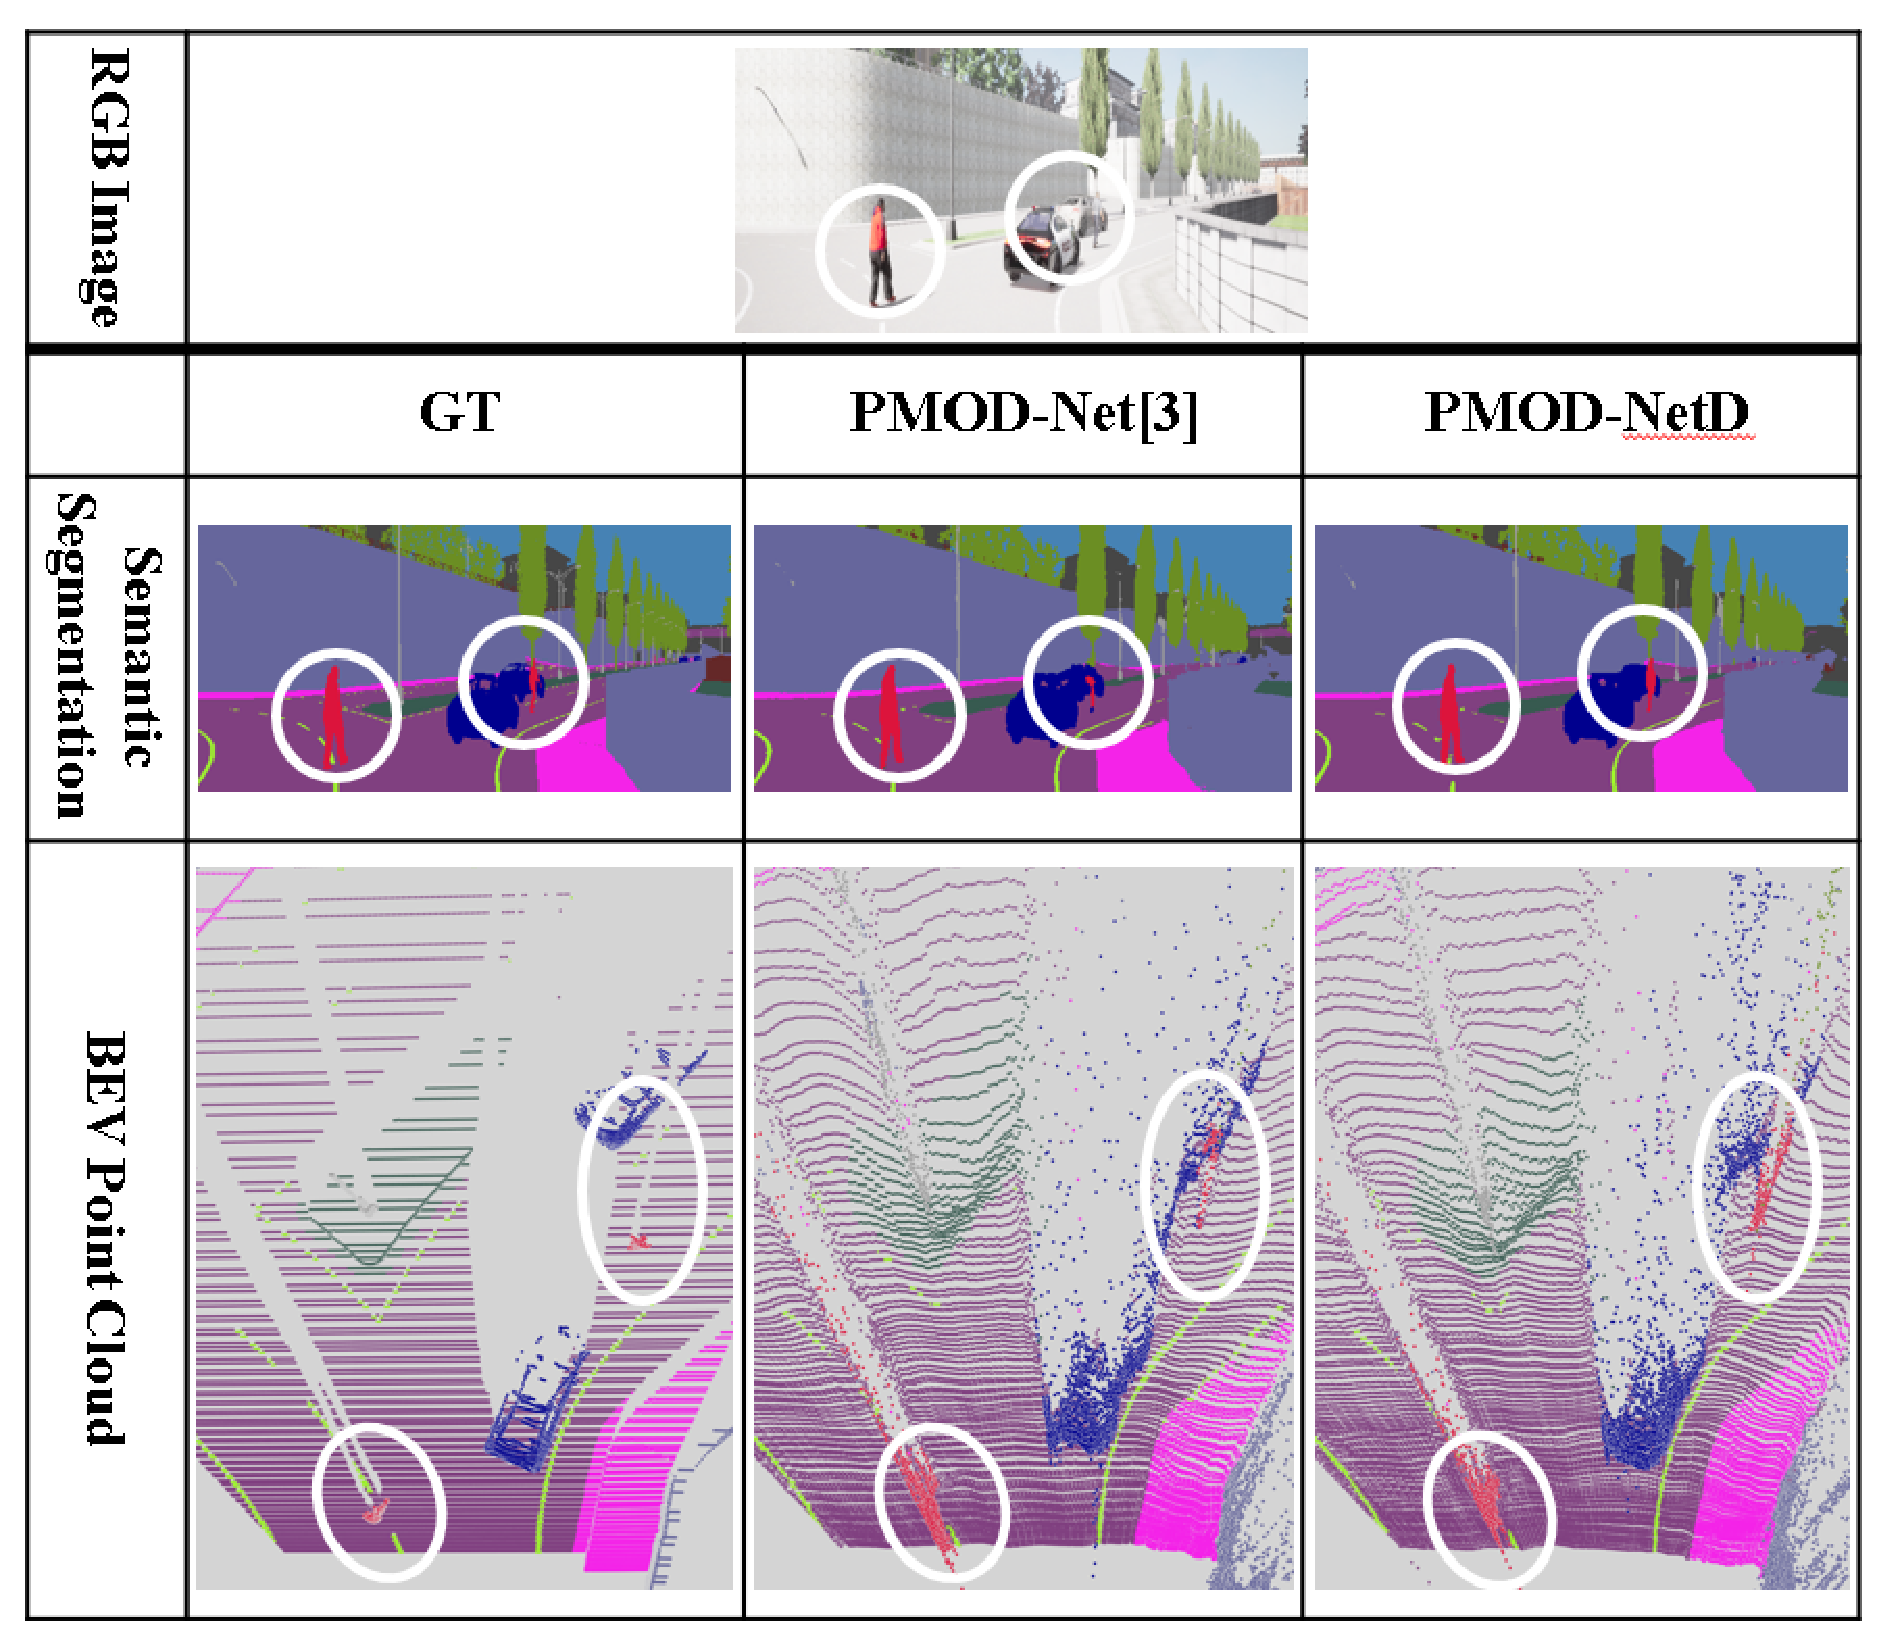
\includegraphics[width=0.935\linewidth]{img/evaluation/result_CARLA.eps}
  \caption{Experimental results in CARLA}
  \label{result_CARLA} 
\end{figure}
\begin{figure}[t]
  \centering
  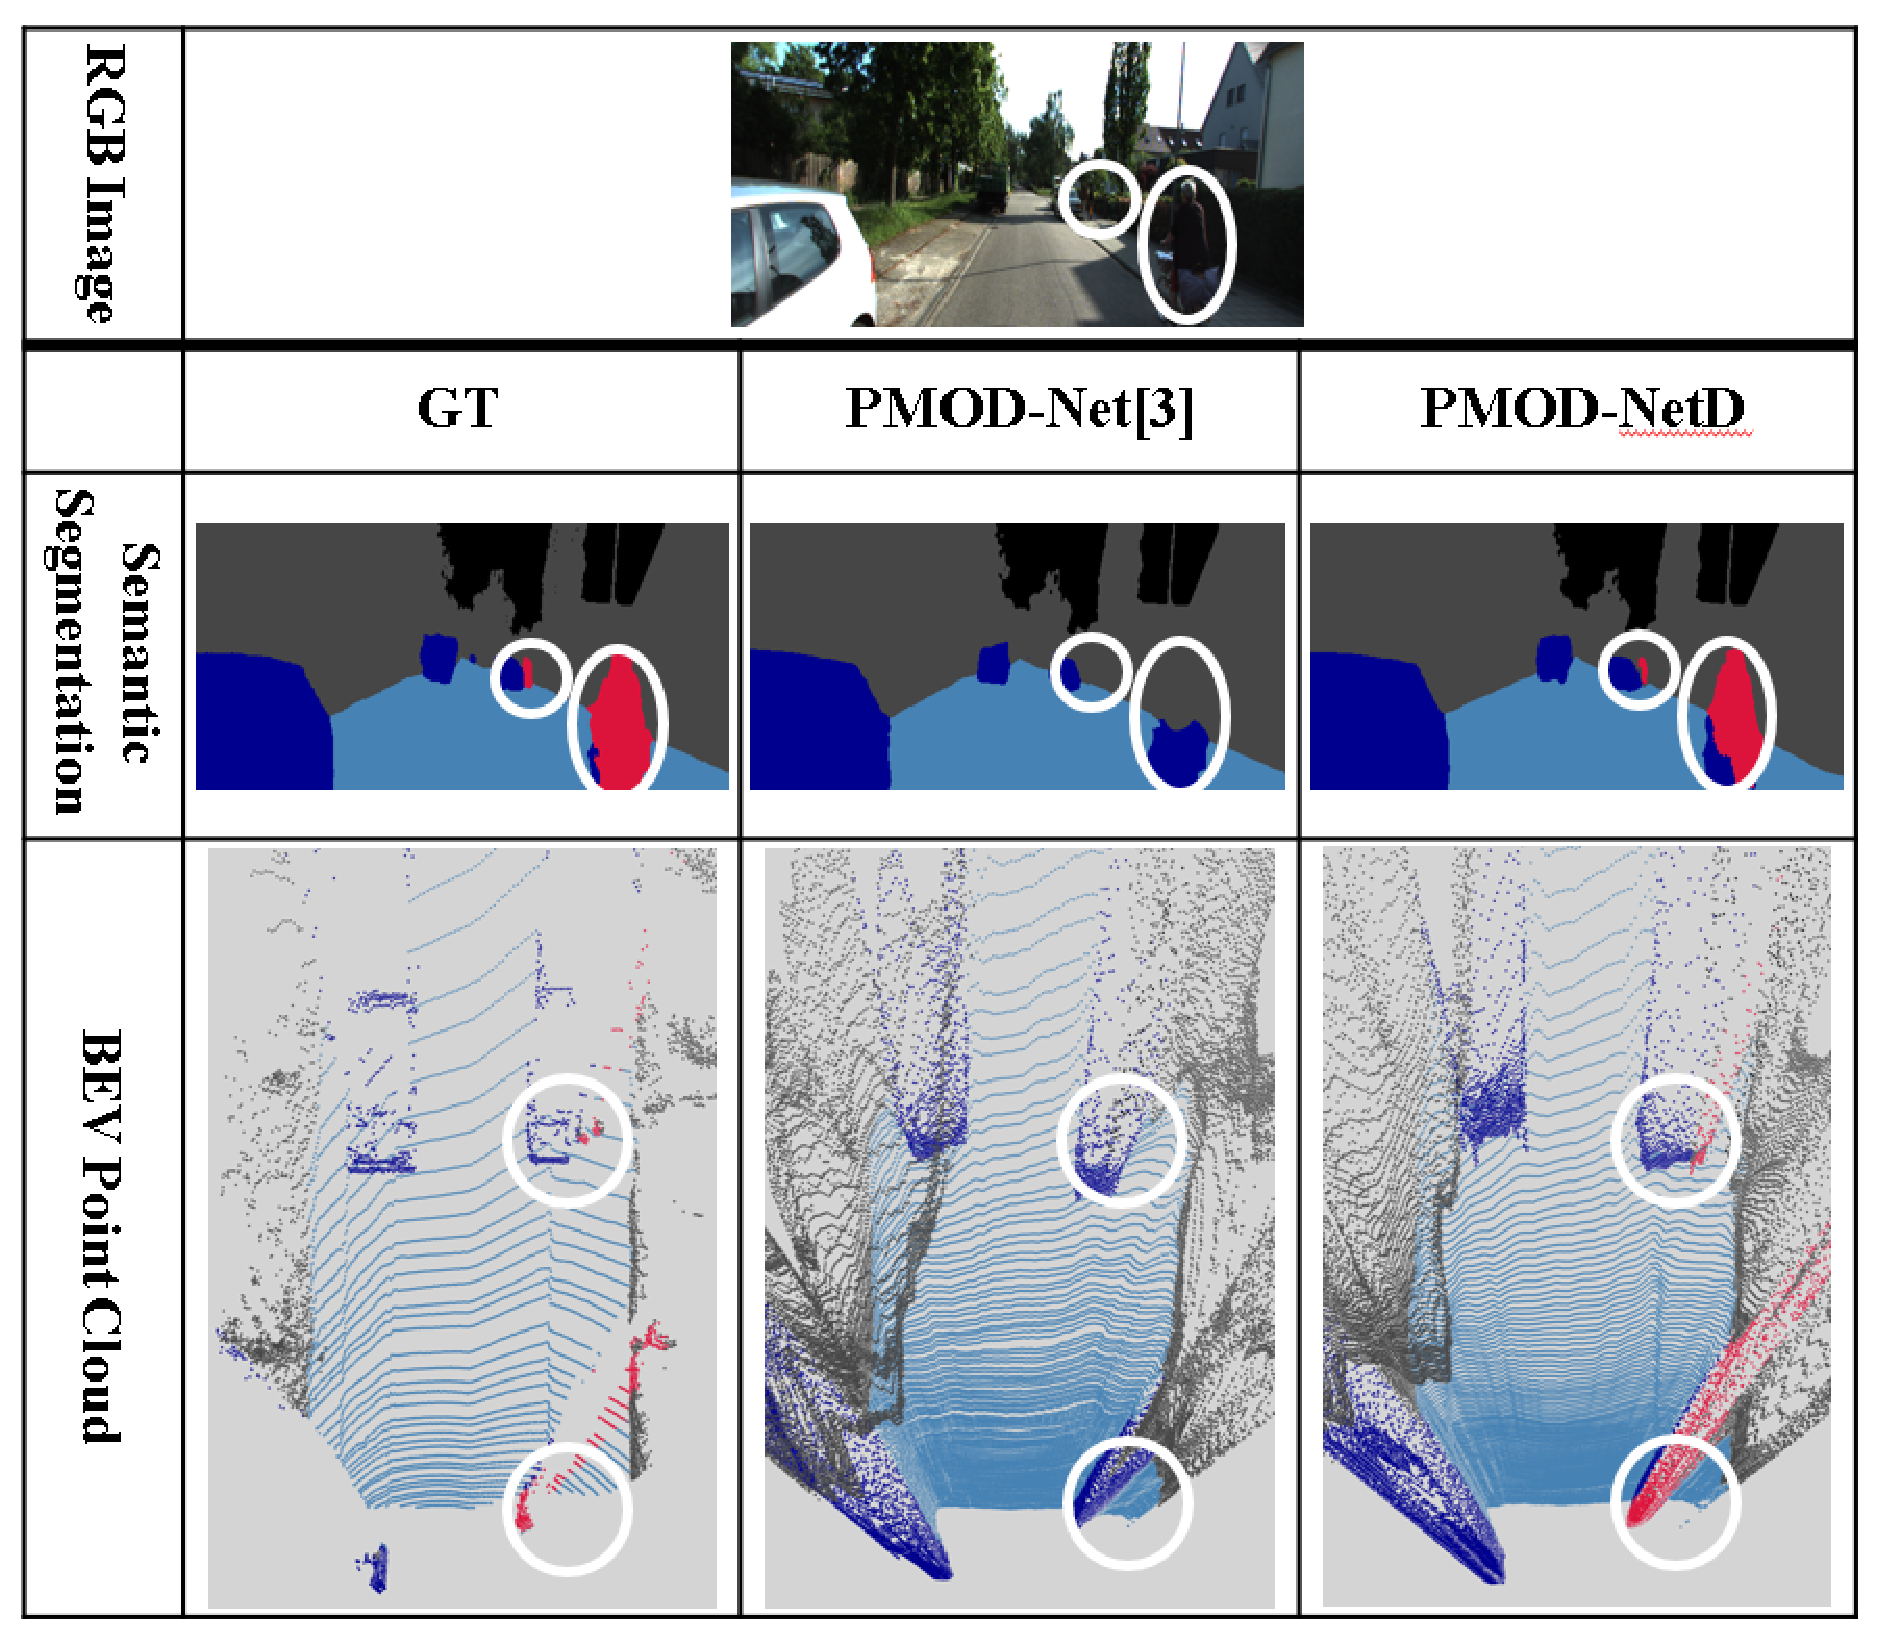
\includegraphics[width=0.935\linewidth]{img/evaluation/result_KITTI-360.eps}
  \caption{Experimental results in KITTI-360}
  \label{result_KITTI-360} 
\end{figure}

\reftable{result_MAE_CARLA}，\reftable{result_MAE_KITTI-360}の実験結果からPMOD-NetDはPMOD-Netよりも精度が向上していることが
わかった．新たに単眼深度画像を導入したことで，動的障害物の
距離推定精度向上に影響を与えたと考える．従来の PMOD-Net
では移動ロボットを利用した低速自動運転において，約2.8m
の間隔で配置された障害物の回避を実現している\cite{3}．本手法はPMOD-Netより精度向上
したため，さらに狭い間隔で障害物が配置された複雑な環境での自動運転に貢献できると
考えられる．

さらに\reffig{result_KITTI-360}のSegmentation結果
を見るとPMOD-Netでは検出できていない人が検出できていることもわかる．
単眼深度推定で障害物の境界を明確にすることは，セグメンテーション結果
にも有用であることが考察された．またNDDepthを用いた場合もMIMDepthを
用いた場合も，元の単眼深度推定結果よりもPMOD-NetDの方が高精度となった．
精度が良いMIMDepthを基にしたPMOD-NetDの方が，より精度が高い．したがって
今後高精度な単眼深度推定が開発された際に，PMOD-NetDに応用することで，
さらなる高精度化が期待できる．

しかし鳥瞰図を見ると，障害物の後方への距離推定誤差がまだ大きいことがわかる．
距離的に遠方にある背景の影響が強いため，障害物の境界を
強調して学習する損失などの導入が必要である．

\reftable{result_ME_CARLA}，\reftable{result_ME_KITTI-360}の実験結果から，本提案手法では，推定位置が正解より手前か奥かといっ
た傾向がデータセットごとに異なることがわかる．データセット内に含まれる物体の距離
の分布によって傾向が異なると考えられるため，手前に推定させたい場合は，データセット
に含まれる物体までの距離を全体的に短くするなど，学習させる距離の分布を調整するこ
とは重要である．


% \section{まとめ}
本研究では，単眼カメラでの距離推定を目的とし，三次元
地図上に存在しない動的障害物の検出精度を向上させるこ
とを目指した．単眼深度推定手法と三次元地図を統合し，動
的障害物の距離を推定するPMOD-NetDを開発した．PMOD-NetDは，公開データセットKITTI-360において人の距離推
定誤差平均は3.25[m]となり，
従来のPMOD-Netより0.85[m]
減少することを確認した．また，KITTIデータセットにおい
て高精度なNDDepthやMIMDepthといった複数の深度推定法
の精度を向上させられる汎用性を持つことが確認された．
今後は，動的障害物の境界に特化した新たな損失を追加し，
障害物回避実験を実施する．
%\section{講演論文原稿作成方法について}
講演論文原稿（PDF形式のみ）の投稿はインターネット経由で行います．
詳細は，第42回日本ロボット学会学術講演会のウェブサイト\cite{website}をご参照ください．原稿は以下の要領で作成してください．

\begin{enumerate}
    \item {\bfseries Microsoft Word の場合}\\
    ウェブサイト\cite{website}から\verb|sample2024j.doc|をダウンロードして講演論文原稿を作成してください．
    MS WordやOSのバージョンによってはレイアウトが崩れる場合があります．
    そうした場合は，適宜\verb|sample2024j.pdf|の書式に合うように原稿を作成してください．

  \item {\bfseries \TeX (pLaTeX/upLaTeX/XeLaTeX) の場合}\\
    ウェブサイト\cite{website}から\verb|sample2024j_tex.zip|をダウンロードし，その中に含まれる\verb|sample2024j.tex| と \verb|rsj2024j.sty|をお使いください．ダウンロードしたものはpLaTeXでコンパイルできる状態になっています．upLaTeXあるいはXeLaTeXをお使いの方は\verb|sample2024j.tex|の先頭部分のコメントアウトされた\verb|documentclass|コマンドをお使いください．
    なお，\TeX では，\verb|sample2024j.pdf|の書式と一部異なる部分があります．ご了承ください．
  \item {\bfseries Typst の場合}\\
    Typst\cite{typst} は\TeX{}に似た新しい組版システムです．RSJ2024ではTypstのテンプレートもご用意いたしました．ウェブサイト\cite{website}から\verb|sample2024j_typst.zip|をダウンロードし，その中に含まれる\verb|sample2024tj.typ|，\verb|samplebib.bib|(参考文献ファイル)および\verb|rsj2024t.typ|(\TeX{}のスタイルファイルのような役割のファイル)をお使いください．
    なお，Typstでは\verb|sample2024j.pdf|の書式と一部異なる部分があります．ご了承ください．
    \item {\bfseries その他の場合}\\        
    \verb|sample2024j.pdf|の書式に合うように原稿を作成してください．
\end{enumerate}

作成したファイル（dviファイル，Wordファイル等）からPDFファイルを作成してください．
このときの画質，セキュリティ，余白等について注意してください．詳細は，ウェブサイト\cite{website}をご参照ください．
また，作成されたPDFファイルを Adobe Acrobat Readerで開いてご確認ください．
確認事項については，ウェブサイト\cite{website}をご参照ください．

\section{講演論文原稿書式について}
\subsection{原稿枚数について}
講演論文原稿は1ページ以上4ページ以内です．
ファイルの容量は3Mバイト（論文参考用動画ファイルを併せてご投稿される場合は，動画ファイルを含めて4Mバイト）までです．
規定ページを超えるものは掲載いたしません．また，容量制限を超えるものは投稿できません．

\subsection{和文原稿の場合}
\subsubsection{原稿の体裁}
A4版白紙に縦250mm，横170mmの枠内に収まるようにお願いします（余白は上側20mm，下側27mm，左右20mm）．
本文は10ポイント程度をご使用ください．
提出された講演論文原稿は，そのまま予稿集に掲載します．
原稿の書き方が不適当にならないようにご留意ください．
詳細については，ウェブサイト\cite{website}をご参照ください．

\subsubsection{図と表について}
図の例を\reffig{fig:sample}に示します．講演論文原稿はPDFファイルとなりますので，図・表はカラーで作成していただいても構いません．
ただし，印刷しても問題ない程度の解像度を持ち，
かつアップロードの際のファイルサイズ上限を越えない大きさとなるようにご留意ください．

%図の入れ方
% \begin{figure}[tb]
%   \centering
%   \large
%   \begin{tikzpicture}
%     \draw rectangle++(4.5,3);
%     \clip rectangle++(4.5,3);
%     \foreach\x in{0,1,2,3,4}{
%       \foreach\y in{0,1,2,3,4,5,6}{
%         \path(\x*1.5-\y*0.5,\y*0.6)node[rotate=10,text=gray]{\sffamily\bfseries\itshape Sample };
%       }
%     }
%   \end{tikzpicture}
  % eps 画像を貼る場合は includegraphics をお使いください．
  % \includegraphics[width=45mm]{samplefig2.eps}
%   \caption{サンプル画像}
%   \label{fig:sample}
% \end{figure}

\subsubsection{参考文献}
文献の引用は本文中に\cite{website}\cite{yamada2000}のように通し番号を付して書き（上付にはしない），参考文献を本文の最後にまとめて書いてください．
参考文献の書式は，日本ロボット学会誌の執筆要項\cite{rsj_rules}に準拠してください．

\subsection{和文原稿の場合の注意点}
学術講演会の和文原稿には，和文題名，和文著者名を掲載してください．
英文題目，英文著者名は併記しないでください．
図中のキャプションや図名も和文とします．

ただし，レター同時投稿オプションを利用する場合は，レター原稿のフォーマットにしたがって和文・英文題目，和文・英文著者名を併記しても構いません．
レター原稿中の図名及び説明文が英語記載となっているため，講演会和文原稿の図名及び説明文も英語で記載しても構いません．

また，2023年より，和文または英文要旨（選択可）の掲載を推奨（レター同時投稿オプションを利用する場合は必須）としています．
要旨は3\textasciitilde6行程度（英文の場合，100語以内）とします．
和文，英文原稿ともキーワードの掲載は必用ありません．

\subsection{英文原稿の場合}
英文原稿の執筆要綱は和文原稿のそれに準じます．
英文による題目，著者名をご記入下さい．
和文による題目，著者名等は不要です．
また，英文で，要旨，本文，図中のキャプションや図名もご記入ください．

\section{講演申し込みおよび電子入稿}
2019 年より講演申し込みと電子入稿の締め切りが異なるものとなり，2 段階での手続きとなりました．
講演申込締切までに，講演題目・著者名・講演概要などを登録し，講演の申し込みをしてください．
その後，論文投稿〆切日までに，講演論文原稿ファイル（PDF 形式）をアップロードしてください．
詳細については，ウェブサイト\cite{website}をご参照ください．

%% 謝辞（必要な場合のみ）
%%\begin{acknowledgements}
%%\end{acknowledgements}

\section{レター同時投稿について}
2020年より，日本ロボット学会学術講演会から日本ロボット学会誌へのレター同時投稿を受け付けています．
日本ロボット学会学術講演会に投稿した講演論文を「そのまま」の内容（フォーマットは異なります）でレター（速報性を有する研究報告．最大 4 ページ）に投稿することが可能ですので，これを同時に受け付けます． 

レター原稿の作成と投稿に関する詳細については，日本ロボット学会誌の規定[3]をご覧頂ければと思いますが，講演会の論文投稿と同時に，ロボット学会ウェブサイトに掲載の論文投稿システムより同内容をレターフォーマットで投稿して頂ければ，査読プロセス（速報性を重視するため初回査読期間は 15 日以内）を経て Acceptされた論文が，講演会後に順次オンラインに掲載されます．

学術講演会等の講演論文を論文誌に投稿する際には「新たな内容の追加や内容の充実が必要である」としていますが，日本ロボット学会が主催する学術講演会については，この規定の対象外としているため，レター同時投稿が可能となっています．
この機会を使って，是非，レター投稿をご検討下さい．

なお，レターは最大4ページですが，4ページ未満の原稿も受け付けます．レター同時投稿の原稿作成ならびに投稿については，ウェブサイト\cite{website}をご参照ください．


%% 謝辞（必要な場合のみ）
%\begin{acknowledgements}
%    Thanks.
%\end{acknowledgements}

%\small
\scriptsize
\begin{thebibliography}{9}
%%%%%%%%%%%%%%%%%%%%%%%%%%%%%%%%%%%%%%%%%%%%%%%%%%%%%%%%%%%%%%%%%%%%%%%%%%%%%%%

\bibitem{website}
``第42回日本ロボット学会学術講演会のウェブサイト''，
  \url{https://ac.rsj-web.org/2024/}
\bibitem{typst}
  ``Typst website'',
  \url{https://typst.app}
\bibitem{yamada2000}
  山田太郎，鈴木一郎：
  ``第100回日本ロボット学会講演会用原稿の書き方''，
  日本ロボット学会誌, vol. 99, no. 4, pp. 8--12, 2082.
\bibitem{rsj_rules}
  ``日本ロボット学会誌・寄稿および査読に関する規則集''，
  \url{https://www.rsj.or.jp/content/files/data_rules/F-02.pdf}
%%%%%%%%%%%%%%%%%%%%%%%%%%%%%%%%%%%%%%%%%%%%%%%%%%%%%%%%%%%%%%%%%%%%%%%%%%%%%%%
\end{thebibliography}

% \section{講演論文原稿作成方法について}
% 講演論文原稿（PDF形式のみ）の投稿はインターネット経由で行います．
% 詳細は，第42回日本ロボット学会学術講演会のウェブサイト\cite{website}をご参照ください．原稿は以下の要領で作成してください．

% \begin{enumerate}
%     \item {\bfseries Microsoft Word の場合}\\
%     ウェブサイト\cite{website}から\verb|sample2024j.doc|をダウンロードして講演論文原稿を作成してください．
%     MS WordやOSのバージョンによってはレイアウトが崩れる場合があります．
%     そうした場合は，適宜\verb|sample2024j.pdf|の書式に合うように原稿を作成してください．

%   \item {\bfseries \TeX (pLaTeX/upLaTeX/XeLaTeX) の場合}\\
%     ウェブサイト\cite{website}から\verb|sample2024j_tex.zip|をダウンロードし，その中に含まれる\verb|sample2024j.tex| と \verb|rsj2024j.sty|をお使いください．ダウンロードしたものはpLaTeXでコンパイルできる状態になっています．upLaTeXあるいはXeLaTeXをお使いの方は\verb|sample2024j.tex|の先頭部分のコメントアウトされた\verb|documentclass|コマンドをお使いください．
%     なお，\TeX では，\verb|sample2024j.pdf|の書式と一部異なる部分があります．ご了承ください．
%   \item {\bfseries Typst の場合}\\
%     Typst\cite{typst} は\TeX{}に似た新しい組版システムです．RSJ2024ではTypstのテンプレートもご用意いたしました．ウェブサイト\cite{website}から\verb|sample2024j_typst.zip|をダウンロードし，その中に含まれる\verb|sample2024tj.typ|，\verb|samplebib.bib|(参考文献ファイル)および\verb|rsj2024t.typ|(\TeX{}のスタイルファイルのような役割のファイル)をお使いください．
%     なお，Typstでは\verb|sample2024j.pdf|の書式と一部異なる部分があります．ご了承ください．
%     \item {\bfseries その他の場合}\\        
%     \verb|sample2024j.pdf|の書式に合うように原稿を作成してください．
% \end{enumerate}

% 作成したファイル（dviファイル，Wordファイル等）からPDFファイルを作成してください．
% このときの画質，セキュリティ，余白等について注意してください．詳細は，ウェブサイト\cite{website}をご参照ください．
% また，作成されたPDFファイルを Adobe Acrobat Readerで開いてご確認ください．
% 確認事項については，ウェブサイト\cite{website}をご参照ください．

% \section{講演論文原稿書式について}
% \subsection{原稿枚数について}
% 講演論文原稿は1ページ以上4ページ以内です．
% ファイルの容量は3Mバイト（論文参考用動画ファイルを併せてご投稿される場合は，動画ファイルを含めて4Mバイト）までです．
% 規定ページを超えるものは掲載いたしません．また，容量制限を超えるものは投稿できません．

% \subsection{和文原稿の場合}
% \subsubsection{原稿の体裁}
% A4版白紙に縦250mm，横170mmの枠内に収まるようにお願いします（余白は上側20mm，下側27mm，左右20mm）．
% 本文は10ポイント程度をご使用ください．
% 提出された講演論文原稿は，そのまま予稿集に掲載します．
% 原稿の書き方が不適当にならないようにご留意ください．
% 詳細については，ウェブサイト\cite{website}をご参照ください．

% \subsubsection{図と表について}
% 図の例を\reffig{fig:sample}に示します．講演論文原稿はPDFファイルとなりますので，図・表はカラーで作成していただいても構いません．
% ただし，印刷しても問題ない程度の解像度を持ち，
% かつアップロードの際のファイルサイズ上限を越えない大きさとなるようにご留意ください．

% %図の入れ方
% \begin{figure}[tb]
%   \centering
%   \large
%   \begin{tikzpicture}
%     \draw rectangle++(4.5,3);
%     \clip rectangle++(4.5,3);
%     \foreach\x in{0,1,2,3,4}{
%       \foreach\y in{0,1,2,3,4,5,6}{
%         \path(\x*1.5-\y*0.5,\y*0.6)node[rotate=10,text=gray]{\sffamily\bfseries\itshape Sample };
%       }
%     }
%   \end{tikzpicture}
%   % eps 画像を貼る場合は includegraphics をお使いください．
%   % \includegraphics[width=45mm]{samplefig2.eps}
%   \caption{サンプル画像}
%   \label{fig:sample}
% \end{figure}

% \subsubsection{参考文献}
% 文献の引用は本文中に\cite{website}\cite{yamada2000}のように通し番号を付して書き（上付にはしない），参考文献を本文の最後にまとめて書いてください．
% 参考文献の書式は，日本ロボット学会誌の執筆要項\cite{rsj_rules}に準拠してください．

% \subsection{和文原稿の場合の注意点}
% 学術講演会の和文原稿には，和文題名，和文著者名を掲載してください．
% 英文題目，英文著者名は併記しないでください．
% 図中のキャプションや図名も和文とします．

% ただし，レター同時投稿オプションを利用する場合は，レター原稿のフォーマットにしたがって和文・英文題目，和文・英文著者名を併記しても構いません．
% レター原稿中の図名及び説明文が英語記載となっているため，講演会和文原稿の図名及び説明文も英語で記載しても構いません．

% また，2023年より，和文または英文要旨（選択可）の掲載を推奨（レター同時投稿オプションを利用する場合は必須）としています．
% 要旨は3\textasciitilde6行程度（英文の場合，100語以内）とします．
% 和文，英文原稿ともキーワードの掲載は必用ありません．

% \subsection{英文原稿の場合}
% 英文原稿の執筆要綱は和文原稿のそれに準じます．
% 英文による題目，著者名をご記入下さい．
% 和文による題目，著者名等は不要です．
% また，英文で，要旨，本文，図中のキャプションや図名もご記入ください．

% \section{講演申し込みおよび電子入稿}
% 2019 年より講演申し込みと電子入稿の締め切りが異なるものとなり，2 段階での手続きとなりました．
% 講演申込締切までに，講演題目・著者名・講演概要などを登録し，講演の申し込みをしてください．
% その後，論文投稿〆切日までに，講演論文原稿ファイル（PDF 形式）をアップロードしてください．
% 詳細については，ウェブサイト\cite{website}をご参照ください．

% %% 謝辞（必要な場合のみ）
% %%\begin{acknowledgements}
% %%\end{acknowledgements}

% \section{レター同時投稿について}
% 2020年より，日本ロボット学会学術講演会から日本ロボット学会誌へのレター同時投稿を受け付けています．
% 日本ロボット学会学術講演会に投稿した講演論文を「そのまま」の内容（フォーマットは異なります）でレター（速報性を有する研究報告．最大 4 ページ）に投稿することが可能ですので，これを同時に受け付けます． 

% レター原稿の作成と投稿に関する詳細については，日本ロボット学会誌の規定[3]をご覧頂ければと思いますが，講演会の論文投稿と同時に，ロボット学会ウェブサイトに掲載の論文投稿システムより同内容をレターフォーマットで投稿して頂ければ，査読プロセス（速報性を重視するため初回査読期間は 15 日以内）を経て Acceptされた論文が，講演会後に順次オンラインに掲載されます．

% 学術講演会等の講演論文を論文誌に投稿する際には「新たな内容の追加や内容の充実が必要である」としていますが，日本ロボット学会が主催する学術講演会については，この規定の対象外としているため，レター同時投稿が可能となっています．
% この機会を使って，是非，レター投稿をご検討下さい．

% なお，レターは最大4ページですが，4ページ未満の原稿も受け付けます．レター同時投稿の原稿作成ならびに投稿については，ウェブサイト\cite{website}をご参照ください．


% %% 謝辞（必要な場合のみ）
% %\begin{acknowledgements}
% %    Thanks.
% %\end{acknowledgements}

% \small
% \begin{thebibliography}{9}
% %%%%%%%%%%%%%%%%%%%%%%%%%%%%%%%%%%%%%%%%%%%%%%%%%%%%%%%%%%%%%%%%%%%%%%%%%%%%%%%

% \bibitem{website}
% ``第42回日本ロボット学会学術講演会のウェブサイト''，
%   \url{https://ac.rsj-web.org/2024/}
% \bibitem{typst}
%   ``Typst website'',
%   \url{https://typst.app}
% \bibitem{yamada2000}
%   山田太郎，鈴木一郎：
%   ``第100回日本ロボット学会講演会用原稿の書き方''，
%   日本ロボット学会誌, vol. 99, no. 4, pp. 8--12, 2082.
% \bibitem{rsj_rules}
%   ``日本ロボット学会誌・寄稿および査読に関する規則集''，
%   \url{https://www.rsj.or.jp/content/files/data_rules/F-02.pdf}
% %%%%%%%%%%%%%%%%%%%%%%%%%%%%%%%%%%%%%%%%%%%%%%%%%%%%%%%%%%%%%%%%%%%%%%%%%%%%%%%
% \end{thebibliography}


\end{document}
